%=====================================================================
%  Trabalho 08 - Reconhecimento de Flores Iris usando MLP
%  EL056 - Redes Neurais Artificiais (PPGEELT/UFU)
%  Compilar dentro da pasta latex/:  pdflatex relatorio_trabalho08 (2x)
%  Resultados: marcadores \textbf{XX,X\%} substituidos automaticamente
%  por latex/resultados_macros.tex (gerado por gerar_macros_latex.py
%  a partir de resultados.json).
%=====================================================================
\documentclass[12pt,a4paper]{article}

%--------------------------- Pacotes ---------------------------------
\usepackage[utf8]{inputenc}
\usepackage[T1]{fontenc}
\IfFileExists{lmodern.sty}{\usepackage{lmodern}}{}
\usepackage[brazil]{babel}
\usepackage[top=3cm,left=3cm,bottom=2cm,right=2cm]{geometry}
\usepackage{setspace}
\usepackage{ragged2e}
\usepackage{graphicx}
\usepackage{amsmath,amssymb}
\usepackage{booktabs}
\usepackage{multirow}
\usepackage{float}
\usepackage{caption}
\usepackage{subcaption}
\usepackage{xcolor}
\usepackage{listings}
\usepackage{upquote}
\usepackage{algorithm}
\usepackage{algpseudocode}
\usepackage{indentfirst}
\usepackage[hidelinks]{hyperref}

\onehalfspacing
\setlength{\parindent}{1.25cm}
\graphicspath{{../figs/}{figs/}}
\captionsetup{font=small,labelfont=bf,justification=centering}
\floatname{algorithm}{Algoritmo}
\renewcommand{\listalgorithmname}{Lista de algoritmos}
\algrenewcommand\algorithmicrequire{\textbf{Entrada:}}
\algrenewcommand\algorithmicensure{\textbf{Saída:}}

\lstset{
  language=Python, basicstyle=\ttfamily\footnotesize, keywordstyle=\color{blue!70!black}\bfseries,
  commentstyle=\color{green!45!black}\itshape, stringstyle=\color{red!60!black},
  numbers=left, numberstyle=\tiny\color{gray}, frame=single, breaklines=true,
  showstringspaces=false, columns=fullflexible, upquote=true, tabsize=4, captionpos=b,
  literate={á}{{\'a}}1 {à}{{\`a}}1 {ã}{{\~a}}1 {â}{{\^a}}1 {é}{{\'e}}1 {ê}{{\^e}}1 {í}{{\'i}}1
           {ó}{{\'o}}1 {ô}{{\^o}}1 {õ}{{\~o}}1 {ú}{{\'u}}1 {ç}{{\c{c}}}1
           {Á}{{\'A}}1 {É}{{\'E}}1 {Í}{{\'I}}1 {Ó}{{\'O}}1 {Ú}{{\'U}}1 {Ç}{{\c{C}}}1
}
\renewcommand{\lstlistingname}{Código}

%--------------------- Bloco de capa ABNT (PPGEELT/UFU) ---------------
%=====================================================================
%  BLOCO REUTILIZAVEL: CAPA + FOLHA DE ROSTO (ABNT NBR 14724)
%  Extraido do modelo fornecido pelo usuario (PPGEELT/UFU).
%  Este arquivo e' pensado para ser colado no preambulo (antes de
%  \begin{document}) de qualquer trabalho que precise da mesma capa.
%=====================================================================

%--------------------------- Logos opcionais --------------------------
\newcommand{\logoou}[2]{%
  \IfFileExists{#1}{\includegraphics[height=#2,width=\linewidth,keepaspectratio]{#1}}%
                   {\rule{0pt}{#2}}}

%=====================================================================
%  >>>>>>>>>>>>>>  PREENCHA AQUI OS DADOS DO TRABALHO  <<<<<<<<<<<<<<
%=====================================================================
\newcommand{\vazio}{}   % marcador interno para campos opcionais -- nao altere

% AJUSTE AQUI conforme necessario:
\newcommand{\Autor}{LUCAS ALBINO MARTINS\\12622EEL006}
\newcommand{\Titulo}{Trabalho 08 - Reconhecimento de Flores Iris usando MLP}
\newcommand{\Subtitulo}{Disciplina: EL056 - Redes Neurais Artificiais}
\newcommand{\Orientador}{Prof. Dr. Keiji Yamanaka}
\newcommand{\Coorientador}{}                    % vazio se nao houver
\newcommand{\Matricula}{}                       % vazio para omitir
\newcommand{\Local}{Uberl\^andia}
\newcommand{\Ano}{2026}

% ---- Titulo do elemento textual (cabecalho da 1a pagina de texto) ----
\newcommand{\TituloTexto}{Classifica\c{c}\~ao do conjunto Iris com Perceptron
Multicamadas, Softmax e Entropia Cruzada}

% ---- Nota de apresentacao da folha de rosto --------------------------
\newcommand{\NotaApresentacao}{%
  Trabalho apresentado ao Programa de P\'os-Gradua\c{c}\~ao em Engenharia
  El\'etrica (PPGEELT) da Universidade Federal de Uberl\^andia como
  requisito parcial de avalia\c{c}\~ao da disciplina.

  \vspace{0.45cm}
  Disciplina: EL056 - Redes Neurais Artificiais.

  \vspace{0.45cm}
  Professor: \Orientador.
  \ifx\Coorientador\vazio\else

    \vspace{0.2cm}
    Coorientador: \Coorientador.
  \fi
}

%--------------------- Logos (pasta figs/, usada tambem para os graficos) ------------
% Caminhos relativos a pasta latex/ (a pasta figs/ fica na raiz do trabalho)
\newcommand{\LogoEsquerda}{../figs/logo-ppgeel.png}
\newcommand{\LogoDireita}{../figs/logo-ufu.png}
\newcommand{\AlturaLogoEsq}{2.2cm}   % ajuste fino da altura de cada logo
\newcommand{\AlturaLogoDir}{2.6cm}

%=====================================================================
%  CABECALHO INSTITUCIONAL (logos + nome da instituicao + filete)
%=====================================================================
\newcommand{\cabecalhoinstitucional}{%
  \begin{center}
    \noindent
    \begin{minipage}[c]{0.19\textwidth}
      \raggedright
      \logoou{\LogoEsquerda}{\AlturaLogoEsq}
    \end{minipage}%
    \hfill
    \begin{minipage}[c]{0.58\textwidth}
      \centering
      \singlespacing
      {\fontsize{12}{15}\selectfont\bfseries
        UNIVERSIDADE FEDERAL DE UBERL\^ANDIA\par}
      \vspace{0.25cm}
      {\fontsize{12}{15}\selectfont
        PPGEELT -- P\'os-Gradua\c{c}\~ao em Engenharia El\'etrica\par}
    \end{minipage}%
    \hfill
    \begin{minipage}[c]{0.19\textwidth}
      \raggedleft
      \logoou{\LogoDireita}{\AlturaLogoDir}
    \end{minipage}

    \vspace{0.35cm}
    \rule{\textwidth}{1.1pt}
  \end{center}
}

%=====================================================================
%  CAPA -- ABNT NBR 14724
%=====================================================================
\newcommand{\fazcapa}{%
  \thispagestyle{empty}
  \begin{center}
    \cabecalhoinstitucional

    \vspace{2.5cm}

    {\fontsize{12}{15}\selectfont\MakeUppercase{\Autor}\par}

    \ifx\Matricula\vazio\else
      \vspace{0.4cm}
      {\fontsize{11}{14}\selectfont Matr\'icula: \Matricula\par}
    \fi

    \vspace{4.0cm}

    {\fontsize{16}{20}\selectfont\bfseries\MakeUppercase{\Titulo}\par}
    \ifx\Subtitulo\vazio\else
      \vspace{0.35cm}
      {\fontsize{13}{16}\selectfont\Subtitulo\par}
    \fi

    \vfill

    {\fontsize{12}{15}\selectfont \Local\par}
    \vspace{0.15cm}
    {\fontsize{12}{15}\selectfont \Ano\par}
  \end{center}
  \newpage
  \setcounter{page}{1}   % a contagem ABNT comeca na folha de rosto
}

%=====================================================================
%  FOLHA DE ROSTO -- ABNT NBR 14724
%=====================================================================
\newcommand{\fazfolhaderosto}{%
  \thispagestyle{empty}
  \begin{center}
    \cabecalhoinstitucional

    \vspace{2.0cm}

    {\fontsize{12}{15}\selectfont\MakeUppercase{\Autor}\par}

    \vspace{3.0cm}

    {\fontsize{16}{20}\selectfont\bfseries\MakeUppercase{\Titulo}\par}
    \ifx\Subtitulo\vazio\else
      \vspace{0.35cm}
      {\fontsize{13}{16}\selectfont\Subtitulo\par}
    \fi
  \end{center}

  \vspace{2.0cm}

  \hfill
  \begin{minipage}{0.5\textwidth}
    \singlespacing
    \setlength{\parindent}{0pt}
    \fontsize{10}{12}\selectfont
    \justifying
    \NotaApresentacao
  \end{minipage}

  \vfill

  \begin{center}
    {\fontsize{12}{15}\selectfont \Local\par}
    \vspace{0.15cm}
    {\fontsize{12}{15}\selectfont \Ano\par}
  \end{center}
  \newpage
}


%=====================================================================
%  MARCADORES DE RESULTADOS (preenchidos via resultados_macros.tex)
%=====================================================================
\newcommand{\XX}{\textbf{XX,X\%}}
\newcommand{\XN}{\textbf{XX}}
\newcommand{\AccTeste}{\XX}      \newcommand{\FUmTeste}{\XX}     \newcommand{\CETeste}{\XN}
\newcommand{\AccVal}{\XX}        \newcommand{\AccTreino}{\XX}
\newcommand{\CETreino}{\XN}      \newcommand{\CEVal}{\XN}
\newcommand{\MelhorEpoca}{\XN}   \newcommand{\EpocasExec}{\XN}   \newcommand{\NParam}{\XN}
\newcommand{\GCSig}{\XN}         \newcommand{\GCTanh}{\XN}       \newcommand{\GCRelu}{\XN}
\newcommand{\PSet}{\XN}\newcommand{\RSet}{\XN}\newcommand{\FSet}{\XN}
\newcommand{\PVer}{\XN}\newcommand{\RVer}{\XN}\newcommand{\FVer}{\XN}
\newcommand{\PVir}{\XN}\newcommand{\RVir}{\XN}\newcommand{\FVir}{\XN}
\newcommand{\PMacro}{\XN}\newcommand{\RMacro}{\XN}\newcommand{\FMacro}{\XN}
\newcommand{\CMTAA}{\XN}\newcommand{\CMTAB}{\XN}\newcommand{\CMTAC}{\XN}
\newcommand{\CMTBA}{\XN}\newcommand{\CMTBB}{\XN}\newcommand{\CMTBC}{\XN}
\newcommand{\CMTCA}{\XN}\newcommand{\CMTCB}{\XN}\newcommand{\CMTCC}{\XN}
\newcommand{\CMKAA}{\XN}\newcommand{\CMKAB}{\XN}\newcommand{\CMKAC}{\XN}
\newcommand{\CMKBA}{\XN}\newcommand{\CMKBB}{\XN}\newcommand{\CMKBC}{\XN}
\newcommand{\CMKCA}{\XN}\newcommand{\CMKCB}{\XN}\newcommand{\CMKCC}{\XN}
\newcommand{\AccKfold}{\XX}      \newcommand{\DPKfold}{\XX}
\newcommand{\FUmKfold}{\XX}      \newcommand{\DPFUmKfold}{\XX}   \newcommand{\FoldsKfold}{\XX}
\newcommand{\ErrosVerVir}{\XN}   \newcommand{\ErrosTotalKfold}{\XN}
\newcommand{\AccTesteLR}{\XX}    \newcommand{\AccKfoldLR}{\XX}   \newcommand{\DPKfoldLR}{\XX}
\newcommand{\AccTesteKNN}{\XX}   \newcommand{\AccKfoldKNN}{\XX}  \newcommand{\DPKfoldKNN}{\XX}
\newcommand{\AccFronteira}{\XX}
\newcommand{\TabelaExperimentos}{%
Neurônios ocultos & 2 / 4 / 8 / 16 / 32 / 10-6 & \XX{} $\pm$ \XX & \XX & \XN \\ \midrule
Taxa $\eta$ & 0,005 / 0,01 / 0,05 / 0,1 / 0,5 & \XX{} $\pm$ \XX & \XX & \XN \\ \midrule
Ativação & sigmoid / tanh / ReLU & \XX{} $\pm$ \XX & \XX & \XN \\}
\newcommand{\TabelaEstatisticas}{%
sepal length & \XN & \XN & \XN & \XN & \XN & 0,7826 \\
sepal width  & \XN & \XN & \XN & \XN & \XN & $-$0,4194 \\
petal length & \XN & \XN & \XN & \XN & \XN & 0,9490 \\
petal width  & \XN & \XN & \XN & \XN & \XN & 0,9565 \\}
% Substitui os marcadores pelos valores reais, se o arquivo existir:
\IfFileExists{resultados_macros.tex}{% Gerado automaticamente por gerar_macros_latex.py -- nao editar.
\renewcommand{\AccTeste}{100,00\%}
\renewcommand{\FUmTeste}{100,00\%}
\renewcommand{\CETeste}{0,0050}
\renewcommand{\AccVal}{100,00\%}
\renewcommand{\AccTreino}{98,10\%}
\renewcommand{\CETreino}{0,0524}
\renewcommand{\CEVal}{0,0402}
\renewcommand{\MelhorEpoca}{99}
\renewcommand{\EpocasExec}{199}
\renewcommand{\NParam}{67}
\renewcommand{\GCSig}{$3{,}0\times10^{-8}$}
\renewcommand{\GCTanh}{$3{,}5\times10^{-8}$}
\renewcommand{\GCRelu}{$1{,}5\times10^{-9}$}
\renewcommand{\PSet}{1,000}
\renewcommand{\RSet}{1,000}
\renewcommand{\FSet}{1,000}
\renewcommand{\PVer}{1,000}
\renewcommand{\RVer}{1,000}
\renewcommand{\FVer}{1,000}
\renewcommand{\PVir}{1,000}
\renewcommand{\RVir}{1,000}
\renewcommand{\FVir}{1,000}
\renewcommand{\PMacro}{1,000}
\renewcommand{\RMacro}{1,000}
\renewcommand{\FMacro}{1,000}
\renewcommand{\CMTAA}{7}
\renewcommand{\CMTAB}{0}
\renewcommand{\CMTAC}{0}
\renewcommand{\CMTBA}{0}
\renewcommand{\CMTBB}{7}
\renewcommand{\CMTBC}{0}
\renewcommand{\CMTCA}{0}
\renewcommand{\CMTCB}{0}
\renewcommand{\CMTCC}{7}
\renewcommand{\AccKfold}{97,33\%}
\renewcommand{\DPKfold}{3,65\%}
\renewcommand{\FUmKfold}{97,32\%}
\renewcommand{\DPFUmKfold}{3,67\%}
\renewcommand{\FoldsKfold}{100,00\%; 93,33\%; 93,33\%; 100,00\%; 100,00\%}
\renewcommand{\CMKAA}{50}
\renewcommand{\CMKAB}{0}
\renewcommand{\CMKAC}{0}
\renewcommand{\CMKBA}{0}
\renewcommand{\CMKBB}{47}
\renewcommand{\CMKBC}{3}
\renewcommand{\CMKCA}{0}
\renewcommand{\CMKCB}{1}
\renewcommand{\CMKCC}{49}
\renewcommand{\ErrosVerVir}{4}
\renewcommand{\ErrosTotalKfold}{4}
\renewcommand{\TabelaExperimentos}{Neurônios ocultos & 2 & 96,67\% $\pm$ 2,36\% & 96,66\% & 607 \\
Neurônios ocultos & 4 & 98,00\% $\pm$ 2,98\% & 98,00\% & 228 \\
Neurônios ocultos & 8 & 97,33\% $\pm$ 3,65\% & 97,32\% & 523 \\
Neurônios ocultos & 16 & 98,00\% $\pm$ 2,98\% & 98,00\% & 263 \\
Neurônios ocultos & 32 & 97,33\% $\pm$ 2,79\% & 97,32\% & 261 \\
Neurônios ocultos & 10-6 & 96,67\% $\pm$ 2,36\% & 96,66\% & 368 \\
\midrule
Taxa $\eta$ & 0,005 & 97,33\% $\pm$ 3,65\% & 97,32\% & 907 \\
Taxa $\eta$ & 0,01 & 97,33\% $\pm$ 3,65\% & 97,32\% & 673 \\
Taxa $\eta$ & 0,05 & 97,33\% $\pm$ 3,65\% & 97,32\% & 523 \\
Taxa $\eta$ & 0,1 & 98,00\% $\pm$ 2,98\% & 97,98\% & 500 \\
Taxa $\eta$ & 0,5 & 95,33\% $\pm$ 1,83\% & 95,31\% & 381 \\
\midrule
Ativação & sigmoid & 97,33\% $\pm$ 3,65\% & 97,32\% & 654 \\
Ativação & tanh & 97,33\% $\pm$ 3,65\% & 97,32\% & 523 \\
Ativação & relu & 96,67\% $\pm$ 3,33\% & 96,66\% & 485 \\}
\renewcommand{\AccTesteLR}{100,00\%}
\renewcommand{\AccKfoldLR}{96,67\%}
\renewcommand{\DPKfoldLR}{3,33\%}
\renewcommand{\AccTesteKNN}{100,00\%}
\renewcommand{\AccKfoldKNN}{94,67\%}
\renewcommand{\DPKfoldKNN}{2,98\%}
\renewcommand{\AccFronteira}{100,00\%}
\renewcommand{\TabelaEstatisticas}{sepal length & 4,3 & 7,9 & 5,843 & 0,828 & 0,7826 & 0,7826 \\
sepal width & 2,0 & 4,4 & 3,057 & 0,436 & -0,4267 & -0,4194 \\
petal length & 1,0 & 6,9 & 3,758 & 1,765 & 0,9490 & 0,9490 \\
petal width & 0,1 & 2,5 & 1,199 & 0,762 & 0,9565 & 0,9565 \\}
}{}

\hypersetup{pdftitle={Trabalho 08 - Reconhecimento de Flores Iris usando MLP},
            pdfauthor={Lucas Albino Martins}}

%=====================================================================
\begin{document}

\fazcapa
\fazfolhaderosto

%----------------------------- Resumo --------------------------------
\begin{center}
  {\bfseries RESUMO}
\end{center}
\begin{singlespace}
\noindent
Este trabalho apresenta o projeto, a implementação e a avaliação de uma rede Perceptron
Multicamadas (MLP) para a classificação das três espécies do conjunto de dados Iris (Fisher, 1936)
a partir de quatro medidas morfológicas. A rede foi implementada do zero em NumPy, com função
Softmax numericamente estável na camada de saída, função de custo entropia cruzada categorial e
retropropagação manual, cujos gradientes foram validados por diferenças finitas (erro relativo
máximo de \GCTanh{} para \textit{tanh}). Adotou-se padronização z-score ajustada apenas no treino,
divisão estratificada 70/15/15, gradiente descendente em mini-batch com momentum e parada antecipada.
A arquitetura 4--8--3 (\textit{tanh}) obteve acurácia de \AccTeste{} no conjunto de teste e de
\AccKfold{} $\pm$ \DPKfold{} na validação cruzada estratificada com cinco partições, desempenho
compatível com a literatura e comparável aos baselines de regressão logística multinomial e
\textit{k}-NN. A \textit{Setosa} é reconhecida sem erros, e as confusões restantes concentram-se no
par \textit{Versicolor}--\textit{Virginica}, que não é linearmente separável.

\vspace{0.5cm}
\noindent\textbf{Palavras-chave:} Redes neurais artificiais. Perceptron multicamadas. Softmax.
Entropia cruzada. Retropropagação. Conjunto Iris.
\end{singlespace}
\newpage

\tableofcontents
\newpage

\begin{center}
  {\large\bfseries \TituloTexto\par}
\end{center}
\vspace{0.5cm}

%=====================================================================
\section{Introdução}
\label{sec:introducao}

O conjunto de dados Iris, publicado por Fisher (1936) para
ilustrar a análise discriminante linear, reúne 150 flores de três espécies do gênero \textit{Iris}
--- \textit{I.~setosa}, \textit{I.~versicolor} e \textit{I.~virginica}, com 50 exemplares cada ---
descritas por quatro medidas em centímetros: comprimento e largura da sépala e da pétala. Ele é um
dos \textit{benchmarks} mais citados em reconhecimento de padrões (DUDA; HART, 1973; DASARATHY, 1980; GATES, 1972) porque
reúne, em escala reduzida, uma classe linearmente separável e um par de classes que não é.

Este trabalho atende ao enunciado do Trabalho~08 da disciplina EL056: treinar uma MLP para
classificar as flores, com função de ativação Softmax na saída e função de custo entropia cruzada.
Para além do mínimo exigido, buscou-se rigor metodológico: implementação sem frameworks de
\textit{deep learning}, verificação numérica dos gradientes, ausência de vazamento de dados no
pré-processamento, avaliação por validação cruzada estratificada, estudo de sensibilidade a
hiperparâmetros e comparação com baselines.

O relatório está organizado da seguinte forma. A Seção~\ref{sec:teoria} apresenta a fundamentação
teórica; a Seção~\ref{sec:dados} descreve a base de dados; a Seção~\ref{sec:metodologia}, a
metodologia; as Seções~\ref{sec:resultados} e \ref{sec:discussao} apresentam e discutem os
resultados; e a Seção~\ref{sec:conclusao} conclui o trabalho.

%=====================================================================
\section{Fundamentação Teórica}
\label{sec:teoria}

\subsection{Perceptron Multicamadas e propagação direta}

Uma MLP com $L$ camadas de pesos mapeia uma entrada $\mathbf{x}\in\mathbb{R}^{d}$ em um vetor de
probabilidades $\hat{\mathbf{y}}\in\mathbb{R}^{K}$. Em notação matricial por lote (cada linha de
$\mathbf{A}^{(0)}=\mathbf{X}\in\mathbb{R}^{N\times d}$ é uma amostra):
\begin{align}
  \mathbf{Z}^{(l)} &= \mathbf{A}^{(l-1)}\mathbf{W}^{(l)} + \mathbf{1}\,\mathbf{b}^{(l)\top},
  && l = 1,\dots,L, \label{eq:z}\\
  \mathbf{A}^{(l)} &= f\big(\mathbf{Z}^{(l)}\big), && l = 1,\dots,L-1, \label{eq:a}\\
  \hat{\mathbf{Y}} &= \operatorname{softmax}\big(\mathbf{Z}^{(L)}\big), \label{eq:saida}
\end{align}
em que $\mathbf{W}^{(l)}\in\mathbb{R}^{n_{l-1}\times n_l}$ e $f$ é a ativação das camadas ocultas:
\begin{equation}
  \sigma(z)=\frac{1}{1+e^{-z}},\qquad \tanh(z)=\frac{e^{z}-e^{-z}}{e^{z}+e^{-z}},\qquad
  \operatorname{ReLU}(z)=\max(0,z), \label{eq:ativacoes}
\end{equation}
com derivadas $\sigma'(z)=\sigma(z)[1-\sigma(z)]$, $\tanh'(z)=1-\tanh^2(z)$ e
$\operatorname{ReLU}'(z)=\mathbb{1}[z>0]$ (HAYKIN, 2001).

\subsection{Função Softmax estável}

A Softmax converte os \textit{logits} $\mathbf{z}\in\mathbb{R}^{K}$ em uma distribuição de
probabilidade:
\begin{equation}
  \hat{y}_k=\frac{e^{z_k}}{\sum_{j=1}^{K} e^{z_j}}
  =\frac{e^{z_k-m}}{\sum_{j=1}^{K} e^{z_j-m}},\qquad m=\max_j z_j. \label{eq:softmax}
\end{equation}
A segunda forma é matematicamente idêntica à primeira, pois o fator $e^{-m}$ se cancela no numerador e
no denominador. Numericamente, porém, ela garante $z_k-m\le 0$, de modo que $e^{z_k-m}\in(0,1]$: não há
\textit{overflow} e pelo menos um termo do denominador vale 1.

\subsection{Entropia cruzada categorial}

Com rótulos codificados em \textit{one-hot} ($y_{nk}=1$ se a amostra $n$ pertence à classe $k$), a
função de custo média é
\begin{equation}
  L=-\frac{1}{N}\sum_{n=1}^{N}\sum_{k=1}^{K} y_{nk}\ln \hat{y}_{nk}, \label{eq:ce}
\end{equation}
que corresponde à log-verossimilhança negativa de um modelo multinomial (GOODFELLOW; BENGIO; COURVILLE, 2016). Na
implementação, $\hat{y}$ é limitado ao intervalo $[\varepsilon,1]$, com $\varepsilon=10^{-12}$, para
evitar $\ln 0$.

\subsection{Gradiente conjunto Softmax + entropia cruzada}

O jacobiano da Softmax é $\partial\hat{y}_k/\partial z_j=\hat{y}_k(\delta_{kj}-\hat{y}_j)$. Para uma
amostra:
\begin{equation}
  \frac{\partial L_n}{\partial z_j}
  =-\sum_{k}\frac{y_k}{\hat{y}_k}\,\hat{y}_k(\delta_{kj}-\hat{y}_j)
  =-y_j+\hat{y}_j\sum_{k}y_k
  =\hat{y}_j-y_j, \label{eq:grad_saida}
\end{equation}
pois $\sum_k y_k=1$. Para o custo médio no lote, $\boldsymbol{\delta}^{(L)}=(\hat{\mathbf{Y}}-\mathbf{Y})/N$.
Esse resultado elimina o cálculo explícito do jacobiano, é numericamente estável e tem gradiente
limitado em $[-1,1]$, o que evita o problema de saturação do erro quadrático com saídas sigmoidais.

\subsection{Retropropagação e regra de atualização}

Aplicando a regra da cadeia de trás para frente (RUMELHART; HINTON; WILLIAMS, 1986; HAYKIN, 2001):
\begin{align}
  \nabla_{\mathbf{W}^{(l)}}L &= \mathbf{A}^{(l-1)\top}\boldsymbol{\delta}^{(l)}, \qquad
  \nabla_{\mathbf{b}^{(l)}}L = \boldsymbol{\delta}^{(l)\top}\mathbf{1}, \label{eq:gradW}\\
  \boldsymbol{\delta}^{(l-1)} &= \big(\boldsymbol{\delta}^{(l)}\mathbf{W}^{(l)\top}\big)\odot
  f'\big(\mathbf{Z}^{(l-1)}\big). \label{eq:delta}
\end{align}
Os parâmetros $\theta$ são atualizados por gradiente descendente em mini-batch com momentum:
\begin{equation}
  \mathbf{v}\leftarrow\mu\,\mathbf{v}-\eta\,\nabla_{\theta}L,\qquad
  \theta\leftarrow\theta+\mathbf{v}, \label{eq:momentum}
\end{equation}
em que $\eta$ é a taxa de aprendizado e $\mu$ o coeficiente de momentum; com $\mu=0$ recupera-se o
gradiente descendente puro.

\subsection{Inicialização dos pesos}

Para manter a variância das ativações e dos gradientes aproximadamente constante entre camadas,
adotou-se a inicialização de Xavier/Glorot (GLOROT; BENGIO, 2010), $W\sim\mathcal{N}\big(0,\,2/(n_{in}+n_{out})\big)$,
para \textit{tanh}, sigmoide e a camada Softmax, e a de He (HE \textit{et al.}, 2015), $W\sim\mathcal{N}(0,\,2/n_{in})$,
para camadas ReLU. Os vieses começam em zero.

%=====================================================================
\section{Base de Dados}
\label{sec:dados}

A base foi fornecida como \texttt{iris\_data.xlsx} (150 linhas $\times$ 5 colunas, sem cabeçalho),
com documentação no arquivo \texttt{iris\_names.txt} do repositório UCI (FISHER, 1988). As colunas 1--4
são os atributos em cm (\textit{sepal length}, \textit{sepal width}, \textit{petal length},
\textit{petal width}), armazenados como texto e convertidos para ponto flutuante; a coluna 5 contém
o rótulo. Não há valores ausentes, e as classes são balanceadas (33,3\% cada). As linhas estão
ordenadas por classe em blocos de 50, o que torna obrigatório embaralhar os dados antes de dividi-los.

\subsection{Correção das amostras 35 e 38}

A documentação registra que duas amostras de \textit{Setosa} divergem do artigo original. Na
planilha, ambas valem $(4{,}9;\,3{,}1;\,1{,}5;\,0{,}1)$; os valores de Fisher são
$(4{,}9;\,3{,}1;\,1{,}5;\,\mathbf{0{,}2})$ para a amostra 35 e $(4{,}9;\,\mathbf{3{,}6};\,\mathbf{1{,}4};\,0{,}1)$
para a 38. Optou-se por \textbf{corrigi-las}, por três razões: os valores verdadeiros são conhecidos e
documentados pela própria fonte, de modo que não se trata de imputação; as duas linhas são idênticas
na planilha, uma duplicata espúria que daria peso dobrado a um único ponto; e a correção restaura a
fidelidade aos dados originais. A decisão é parametrizável (\texttt{--corrigir-uci} /
\texttt{CORRIGIR\_UCI}) e tem efeito desprezível sobre o desempenho, pois ambas as amostras pertencem
à classe separável.

\subsection{Análise exploratória}

A Tabela~\ref{tab:estatisticas} compara as estatísticas calculadas (após a correção) com as
documentadas. Sem a correção, os valores reproduzem exatamente a documentação; com ela, apenas
\textit{sepal width} se altera de forma perceptível, por ser o atributo modificado na amostra 38.

\begin{table}[H]
  \centering
  \caption{Estatísticas dos atributos (cm), desvio-padrão amostral e correlação de Pearson com o
  rótulo (0, 1, 2).}
  \label{tab:estatisticas}
  \small
  \begin{tabular}{lcccccc}
    \toprule
    Atributo & Mín. & Máx. & Média & DP & Corr. (calc.) & Corr. (UCI) \\
    \midrule
    \TabelaEstatisticas
    \bottomrule
  \end{tabular}
\end{table}

As Figuras~\ref{fig:scatter} e \ref{fig:boxplots} confirmam o que a documentação aponta: as medidas
de pétala são as mais discriminantes, com correlação com a classe de cerca de 0,95. No plano das
pétalas, a \textit{Setosa} forma um aglomerado isolado, enquanto \textit{Versicolor} e
\textit{Virginica} se sobrepõem parcialmente. A Figura~\ref{fig:correlacao} mostra ainda a forte
colinearidade entre \textit{petal length}, \textit{petal width} e \textit{sepal length}.

\begin{figure}[H]
  \centering
  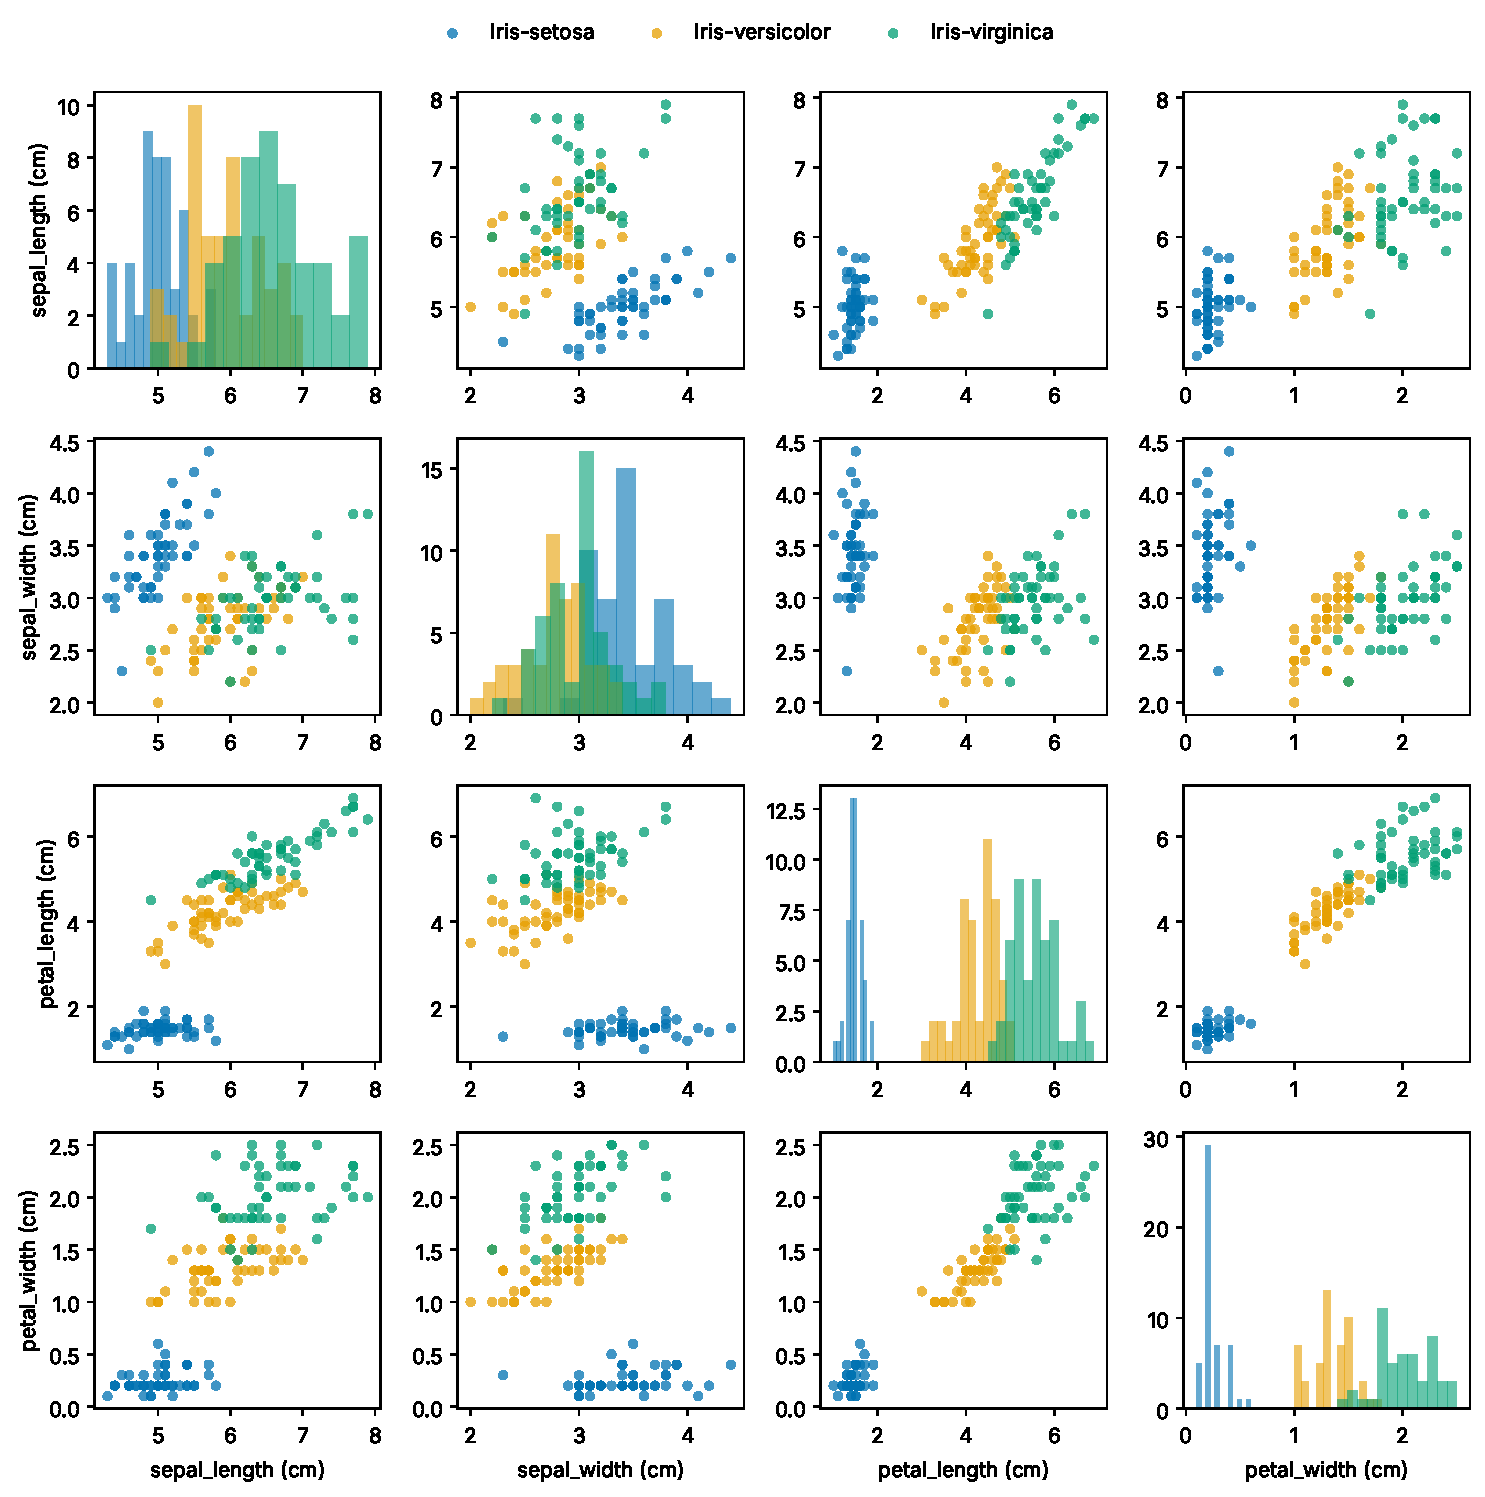
\includegraphics[width=0.82\textwidth]{scatter_matrix.pdf}
  \caption{Matriz de dispersão dos quatro atributos, colorida por classe (diagonal: histogramas).}
  \label{fig:scatter}
\end{figure}

\begin{figure}[H]
  \centering
  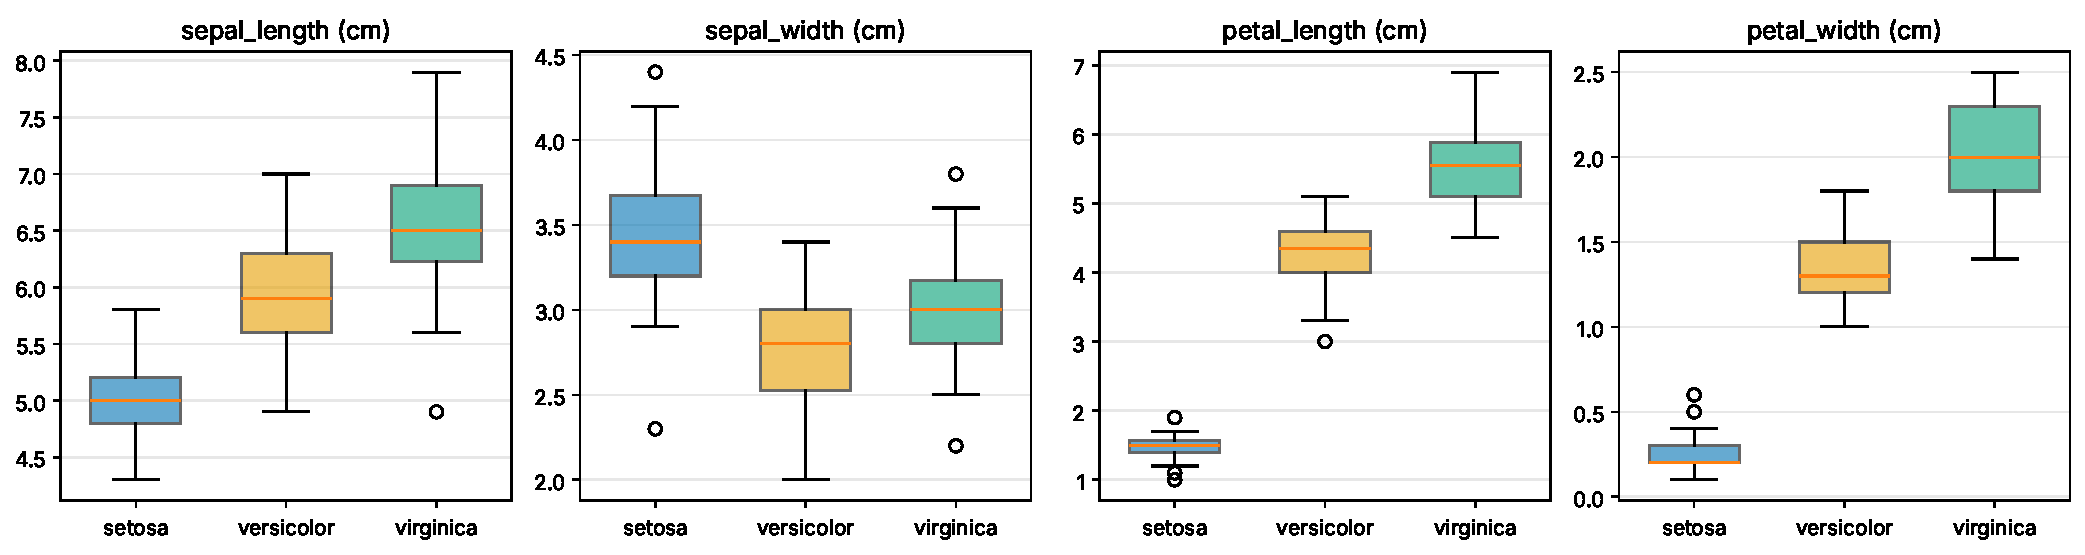
\includegraphics[width=\textwidth]{boxplots.pdf}
  \caption{Distribuição de cada atributo por classe.}
  \label{fig:boxplots}
\end{figure}

\begin{figure}[H]
  \centering
  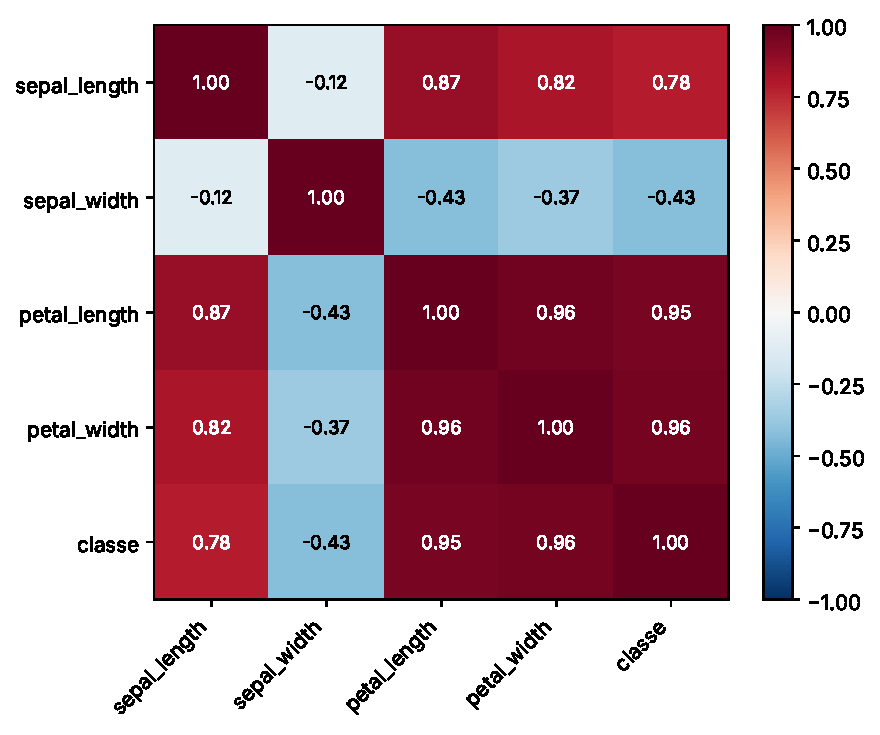
\includegraphics[width=0.55\textwidth]{correlacao.pdf}
  \caption{Correlação de Pearson entre atributos e rótulo.}
  \label{fig:correlacao}
\end{figure}

%=====================================================================
\section{Metodologia}
\label{sec:metodologia}

\subsection{Pré-processamento e divisão dos dados}

Os rótulos foram codificados em \textit{one-hot}. Para o holdout, adotou-se uma divisão estratificada
70/15/15 com semente fixa (\texttt{SEED = 42}). O arredondamento por classe resulta em 35/8/7
amostras por espécie, ou 105/24/21 no total. O conjunto de validação é usado exclusivamente para a
parada antecipada, e o de teste, apenas na avaliação final. Os atributos foram padronizados por
z-score, $x'=(x-\mu_{\text{treino}})/\sigma_{\text{treino}}$, com média e desvio estimados
\textbf{somente no treino} e aplicados à validação e ao teste, evitando vazamento de informação.

Como 21 amostras de teste produzem uma estimativa de alta variância (cada erro vale cerca de 4,8 pontos
percentuais), o desempenho também foi avaliado por validação cruzada \textbf{k-fold estratificada}
com $k=5$. Em cada partição, 15\% da parte de treino é separada, de forma estratificada, para a parada
antecipada, e o z-score é reajustado sobre os 85\% restantes.

\subsection{Arquitetura e hiperparâmetros}

A Tabela~\ref{tab:config} resume a configuração principal. A escolha de \textbf{uma camada oculta}
apoia-se no teorema da aproximação universal e na simplicidade do problema, cuja única fronteira
difícil (\textit{Versicolor}/\textit{Virginica}) é quase linear. \textbf{Oito neurônios} dão folga
sobre o mínimo necessário sem super-parametrizar as 105 amostras de treino; essa hipótese é testada
na Seção~\ref{sec:experimentos}. A \textbf{tangente hiperbólica} foi escolhida por ser centrada em
zero, o que produz gradientes mais bem condicionados que os da sigmoide, e por ser compatível com a
inicialização de Xavier. O mini-batch de 16 amostras resulta em cerca de 7 atualizações por época, e
o ruído estocástico ajuda a escapar de platôs. O momentum de 0,9 acelera a descida em direções de
curvatura baixa.

\begin{table}[H]
  \centering
  \caption{Configuração principal da MLP.}
  \label{tab:config}
  \small
  \begin{tabular}{ll}
    \toprule
    Item & Valor \\
    \midrule
    Arquitetura & 4 -- 8 (\textit{tanh}) -- 3 (Softmax), \NParam{} parâmetros \\
    Inicialização & Xavier/Glorot (vieses nulos) \\
    Custo & Entropia cruzada categorial, Eq.~\eqref{eq:ce} \\
    Otimizador & SGD em mini-batch, $\eta=0{,}05$, $\mu=0{,}9$, lote = 16 \\
    Parada antecipada & até 2000 épocas, paciência = 100 (perda de validação) \\
    Semente & 42 \\
    \bottomrule
  \end{tabular}
\end{table}

\subsection{Algoritmo de treinamento}

O Algoritmo~\ref{alg:treino} sintetiza o procedimento implementado na função \texttt{treinar}.

\begin{algorithm}[H]
  \caption{Treinamento da MLP com mini-batch, momentum e parada antecipada}
  \label{alg:treino}
  \begin{algorithmic}[1]
    \Require $(\mathbf{X}_{tr},\mathbf{Y}_{tr})$, $(\mathbf{X}_{va},\mathbf{Y}_{va})$, $\eta$, $\mu$,
             lote $B$, $E_{\max}$, paciência $P$
    \Ensure pesos $\theta^\star$ da melhor época
    \State Inicializar $\mathbf{W}^{(l)}$ (Xavier/He), $\mathbf{b}^{(l)}\gets\mathbf{0}$, $\mathbf{v}\gets\mathbf{0}$
    \State $L^\star\gets\infty$; \ $p\gets 0$
    \For{$e = 1$ \textbf{até} $E_{\max}$}
      \State Embaralhar índices de treino
      \For{cada lote $\mathcal{B}$ de tamanho $B$}
        \State $\hat{\mathbf{Y}}_{\mathcal{B}}\gets$ \Call{Forward}{$\mathbf{X}_{\mathcal{B}}$} \Comment{Eqs.~\eqref{eq:z}--\eqref{eq:saida}}
        \State $\boldsymbol{\delta}^{(L)}\gets(\hat{\mathbf{Y}}_{\mathcal{B}}-\mathbf{Y}_{\mathcal{B}})/|\mathcal{B}|$ \Comment{Eq.~\eqref{eq:grad_saida}}
        \State Retropropagar $\boldsymbol{\delta}$ e obter $\nabla_\theta L$ \Comment{Eqs.~\eqref{eq:gradW}--\eqref{eq:delta}}
        \State $\mathbf{v}\gets\mu\mathbf{v}-\eta\nabla_\theta L$; \ $\theta\gets\theta+\mathbf{v}$ \Comment{Eq.~\eqref{eq:momentum}}
      \EndFor
      \State Calcular $L_{va}$ e acurácias de treino/validação; registrar histórico
      \If{$L_{va} < L^\star - 10^{-6}$}
        \State $L^\star\gets L_{va}$; \ $\theta^\star\gets\theta$; \ $p\gets 0$
      \Else
        \State $p\gets p+1$; \ \textbf{se} $p\ge P$ \textbf{então interromper}
      \EndIf
    \EndFor
    \State \Return $\theta^\star$
  \end{algorithmic}
\end{algorithm}

\subsection{Verificação do gradiente}

Antes do treinamento, o gradiente analítico foi comparado ao numérico, obtido por diferenças centrais
($\epsilon=10^{-5}$) em todos os parâmetros de uma rede 4--5--4--3. A rede tem duas camadas ocultas
para exercitar a recursão da Eq.~\eqref{eq:delta}. O critério de aceitação é
$|g_a-g_n|/\max(|g_a|+|g_n|,10^{-12})<10^{-6}$.

\subsection{Experimentos e baselines}
\label{sec:experimentos}

Em torno da configuração base, variou-se um fator por vez, com avaliação por k-fold ($k=5$): número de
neurônios ocultos $\{2, 4, 8, 16, 32, (10,6)\}$, taxa de aprendizado
$\{0{,}005;\ 0{,}01;\ 0{,}05;\ 0{,}1;\ 0{,}5\}$ e ativação $\{\text{sigmoide}, \tanh, \text{ReLU}\}$.
Como baselines, usaram-se a regressão logística multinomial, equivalente a uma rede Softmax sem
camada oculta e, portanto, uma medida direta do ganho trazido pela não linearidade, e o
\textit{k}-NN com $k=5$ (DASARATHY, 1980; GATES, 1972), ambos do scikit-learn, sobre os mesmos splits e
partições. Treinou-se ainda uma MLP auxiliar apenas com os atributos de pétala, para visualizar a
fronteira de decisão em duas dimensões.

\subsection{Métricas}

Para cada classe $c$: precisão $P_c=TP_c/(TP_c+FP_c)$, revocação $R_c=TP_c/(TP_c+FN_c)$ e
$F1_c=2P_cR_c/(P_c+R_c)$, além das médias \textit{macro}, da acurácia global e das matrizes de
confusão.

%=====================================================================
\section{Resultados}
\label{sec:resultados}

Todos os valores desta seção foram gerados por \texttt{iris\_mlp.py} (registrados em
\texttt{resultados.json}). O notebook \texttt{iris\_mlp.ipynb} reproduz os mesmos números.

\subsection{Verificação do gradiente}

O erro relativo máximo entre gradiente analítico e numérico foi \GCSig{} (sigmoide), \GCTanh{}
(\textit{tanh}) e \GCRelu{} (ReLU), todos abaixo do limiar de $10^{-6}$. A implementação da
retropropagação, incluindo a Eq.~\eqref{eq:grad_saida}, está correta.

\subsection{Treinamento}

A Figura~\ref{fig:curvas} mostra as curvas de aprendizado. A parada antecipada selecionou a época
\MelhorEpoca{}, de um total de \EpocasExec{} épocas executadas. Nessa época, a entropia cruzada foi de
\CETreino{} no treino e \CEVal{} na validação, com acurácias de \AccTreino{} e \AccVal{},
respectivamente.

\begin{figure}[H]
  \centering
  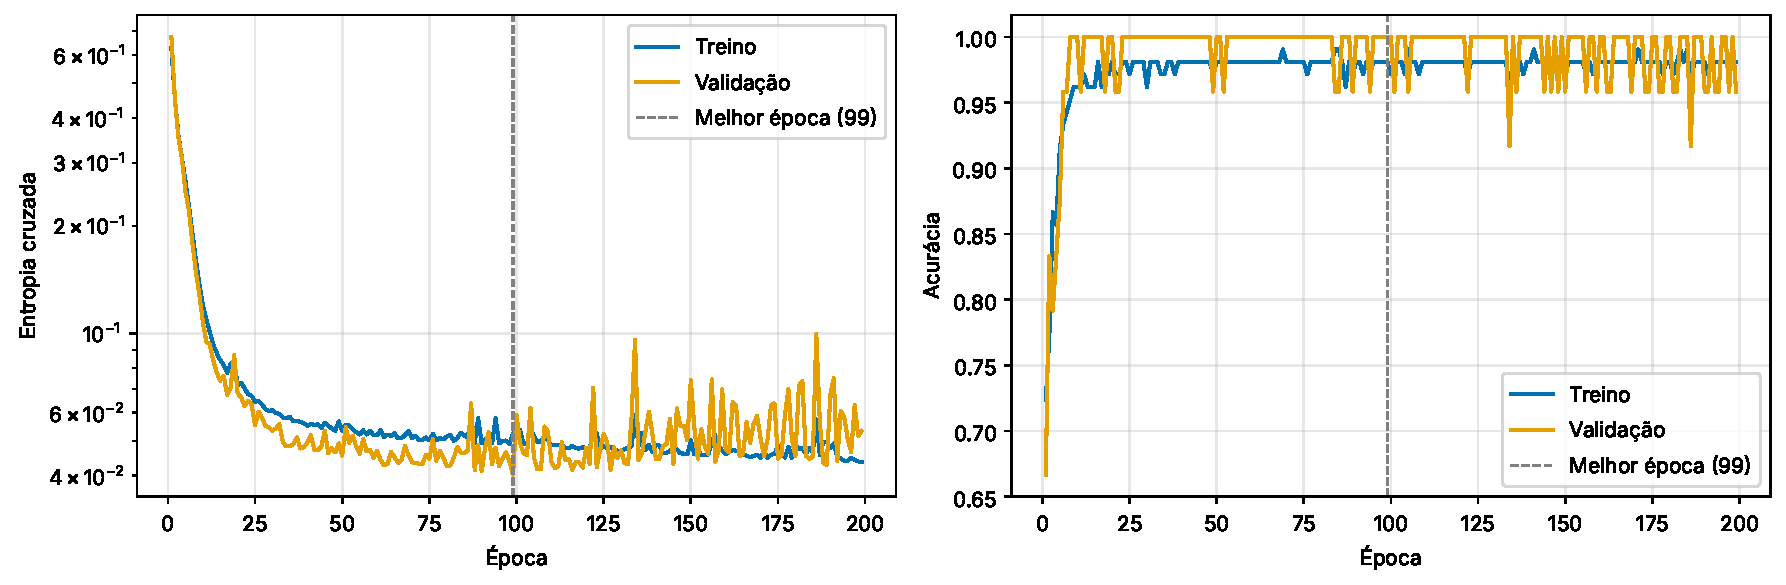
\includegraphics[width=\textwidth]{curvas_treino.pdf}
  \caption{Curvas de perda (escala logarítmica) e de acurácia de treino e validação; a linha
  tracejada indica a época restaurada pela parada antecipada.}
  \label{fig:curvas}
\end{figure}

\subsection{Desempenho no conjunto de teste}

No conjunto de teste (21 amostras), a MLP obteve acurácia de \AccTeste{}, F1 macro de \FUmTeste{}
e entropia cruzada de \CETeste{}. As Tabelas~\ref{tab:metricas} e \ref{tab:cm} e a
Figura~\ref{fig:cm} detalham os resultados.

\begin{table}[H]
  \centering
  \caption{Métricas por classe no conjunto de teste.}
  \label{tab:metricas}
  \small
  \begin{tabular}{lccc}
    \toprule
    Classe & Precisão & Revocação & F1 \\
    \midrule
    \textit{Iris setosa}     & \PSet & \RSet & \FSet \\
    \textit{Iris versicolor} & \PVer & \RVer & \FVer \\
    \textit{Iris virginica}  & \PVir & \RVir & \FVir \\
    \midrule
    Média macro & \PMacro & \RMacro & \FMacro \\
    \bottomrule
  \end{tabular}
\end{table}

\begin{table}[H]
  \centering
  \caption{Matrizes de confusão (linhas: classe real; colunas: classe prevista).}
  \label{tab:cm}
  \small
  \begin{tabular}{lccc@{\hspace{1.2cm}}ccc}
    \toprule
    & \multicolumn{3}{c}{Teste (holdout, $n=21$)} & \multicolumn{3}{c}{k-fold agregado ($n=150$)} \\
    \cmidrule(lr){2-4}\cmidrule(lr){5-7}
    Real $\backslash$ Prevista & Set. & Ver. & Vir. & Set. & Ver. & Vir. \\
    \midrule
    Setosa     & \CMTAA & \CMTAB & \CMTAC & \CMKAA & \CMKAB & \CMKAC \\
    Versicolor & \CMTBA & \CMTBB & \CMTBC & \CMKBA & \CMKBB & \CMKBC \\
    Virginica  & \CMTCA & \CMTCB & \CMTCC & \CMKCA & \CMKCB & \CMKCC \\
    \bottomrule
  \end{tabular}
\end{table}

\begin{figure}[H]
  \centering
  \begin{subfigure}{0.48\textwidth}
    \centering
    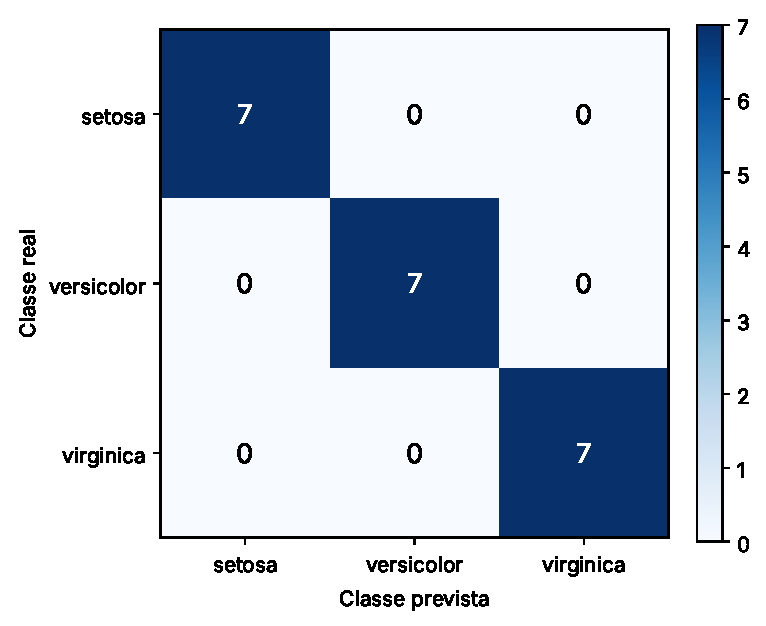
\includegraphics[width=\linewidth]{matriz_confusao.pdf}
    \caption{Teste (holdout).}
  \end{subfigure}\hfill
  \begin{subfigure}{0.48\textwidth}
    \centering
    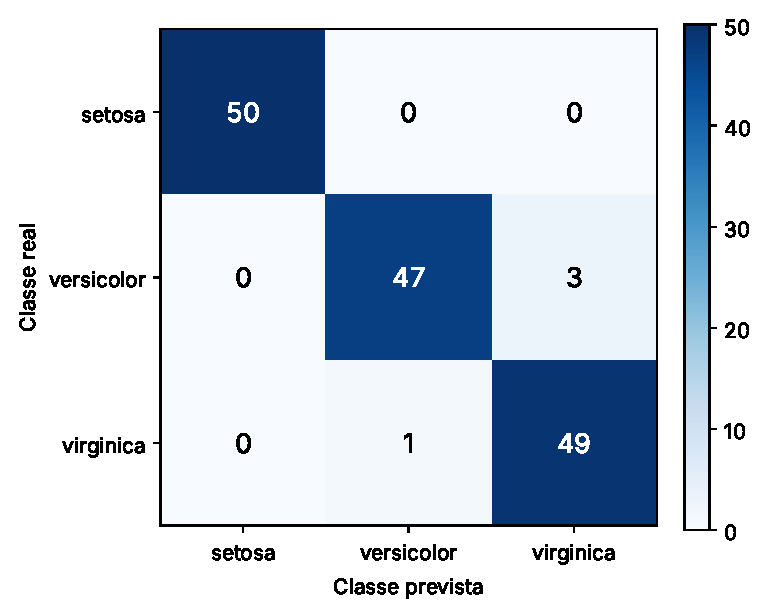
\includegraphics[width=\linewidth]{matriz_confusao_kfold.pdf}
    \caption{k-fold agregado (predições fora da partição).}
  \end{subfigure}
  \caption{Matrizes de confusão da MLP 4--8--3.}
  \label{fig:cm}
\end{figure}

\subsection{Validação cruzada e experimentos}

Com $k=5$, a configuração principal obteve acurácia de \AccKfold{} $\pm$ \DPKfold{} e F1 macro de
\FUmKfold{} $\pm$ \DPFUmKfold{}. As acurácias por partição foram \FoldsKfold. A
Tabela~\ref{tab:experimentos} e a Figura~\ref{fig:experimentos} apresentam o estudo de sensibilidade.

\begin{table}[H]
  \centering
  \caption{Sensibilidade a hiperparâmetros (k-fold estratificado, $k=5$; média $\pm$ desvio-padrão).
  Os demais hiperparâmetros seguem a Tabela~\ref{tab:config}.}
  \label{tab:experimentos}
  \small
  \begin{tabular}{llccc}
    \toprule
    Fator & Valor & Acurácia & F1 macro & Melhor época (média) \\
    \midrule
    \TabelaExperimentos
    \bottomrule
  \end{tabular}
\end{table}

\begin{figure}[H]
  \centering
  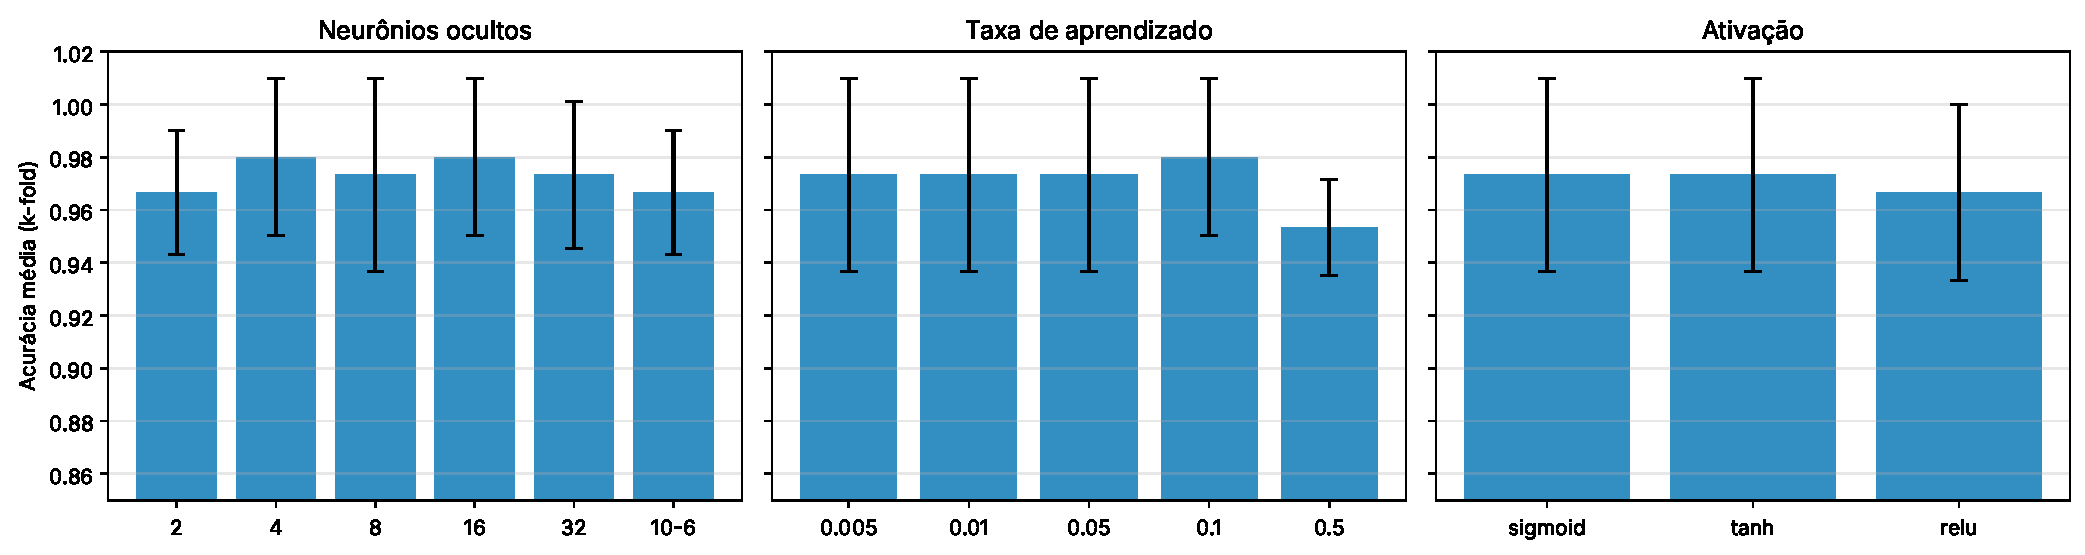
\includegraphics[width=\textwidth]{experimentos.pdf}
  \caption{Acurácia média do k-fold ($\pm$ desvio-padrão) para cada fator variado.}
  \label{fig:experimentos}
\end{figure}

\subsection{Comparação com baselines}

\begin{table}[H]
  \centering
  \caption{Comparação com baselines (mesmo split holdout e mesmas partições do k-fold).}
  \label{tab:baselines}
  \small
  \begin{tabular}{lcc}
    \toprule
    Modelo & Acurácia (teste) & Acurácia k-fold \\
    \midrule
    MLP 4--8--3 (\textit{tanh}, Softmax + CE) & \AccTeste & \AccKfold{} $\pm$ \DPKfold \\
    Regressão logística multinomial & \AccTesteLR & \AccKfoldLR{} $\pm$ \DPKfoldLR \\
    \textit{k}-NN ($k=5$) & \AccTesteKNN & \AccKfoldKNN{} $\pm$ \DPKfoldKNN \\
    \bottomrule
  \end{tabular}
\end{table}

\subsection{Fronteira de decisão}

A MLP auxiliar treinada apenas com \textit{petal length} e \textit{petal width} obteve acurácia de
teste de \AccFronteira. Suas regiões de decisão aparecem na Figura~\ref{fig:fronteira}.

\begin{figure}[H]
  \centering
  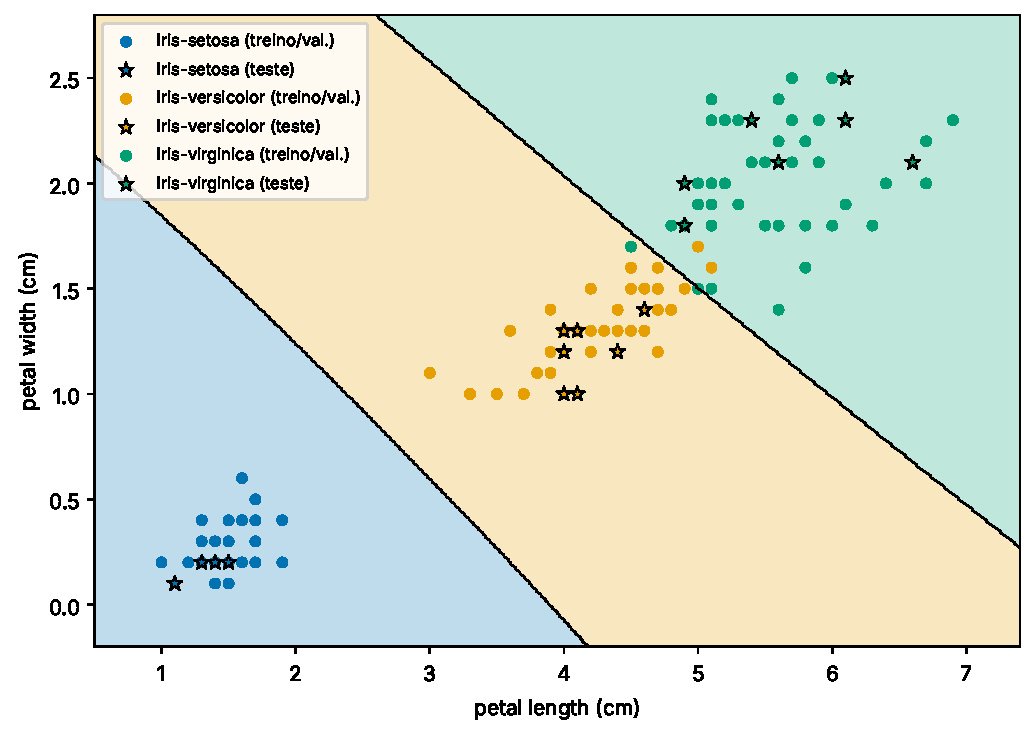
\includegraphics[width=0.75\textwidth]{fronteira_decisao.pdf}
  \caption{Regiões de decisão da MLP no plano das pétalas; as estrelas indicam as amostras de teste.}
  \label{fig:fronteira}
\end{figure}

%=====================================================================
\section{Discussão}
\label{sec:discussao}

\textbf{Correção da implementação.} O \textit{gradient checking} confirma que a retropropagação
manual, incluindo a simplificação $\partial L/\partial\mathbf{z}=\hat{\mathbf{y}}-\mathbf{y}$, está
correta para as três ativações. Esse teste é o que dá confiabilidade a uma implementação feita do
zero: sem ele, erros sutis de sinal ou de dimensão podem passar despercebidos, porque a rede às vezes
"aprende" mesmo com gradientes incorretos.

\textbf{Dinâmica de treinamento.} As curvas da Figura~\ref{fig:curvas} mostram queda rápida da perda
nas primeiras épocas, seguida de estabilização. A perda de validação passa a oscilar em torno do
mínimo, efeito do ruído do mini-batch e do tamanho reduzido do conjunto de validação. A parada
antecipada restaura os pesos de menor perda de validação, o que funciona como regularização
implícita.

\textbf{Holdout versus k-fold.} Com 7 amostras por classe no teste, a acurácia holdout
(\AccTeste) tem alta variância e não deve ser lida isoladamente. A estimativa de referência é a do
k-fold (\AccKfold{} $\pm$ \DPKfold), cujo desvio-padrão quantifica a variabilidade entre partições.

\textbf{Confusão \textit{Versicolor} $\times$ \textit{Virginica}.} A matriz agregada do k-fold
(Tabela~\ref{tab:cm}) mostra que a \textit{Setosa} não é confundida com nenhuma outra classe, o que é
coerente com sua separabilidade linear. Dos \ErrosTotalKfold{} erros fora da partição,
\ErrosVerVir{} ocorrem entre \textit{Versicolor} e \textit{Virginica}. A Figura~\ref{fig:fronteira}
mostra a causa: as duas espécies se sobrepõem na região de pétalas intermediárias (comprimento de
cerca de 4,5 a 5,1~cm e largura de 1,5 a 1,8~cm). Nessa região, amostras de classes distintas têm
medidas praticamente iguais, e o erro é essencialmente irredutível com esses quatro atributos.

\textbf{Sensibilidade a hiperparâmetros.} Na faixa avaliada, as variações de arquitetura, taxa de
aprendizado e ativação produzem diferenças de desempenho da ordem do desvio-padrão entre partições
(Tabela~\ref{tab:experimentos}), ou seja, sem diferença estatisticamente relevante. Taxas menores
exigem mais épocas até o mínimo de validação, e taxas muito altas tornam a otimização mais ruidosa.
Redes com 2 neurônios já são suficientes, o que confirma que a fronteira necessária é simples. A
escolha de 8 neurônios com \textit{tanh} é, portanto, adequada, mas não crítica.

\textbf{MLP versus baselines.} A regressão logística multinomial, que é uma rede Softmax sem camada
oculta, atinge desempenho próximo ao da MLP (Tabela~\ref{tab:baselines}), indicando que o problema é
quase linearmente separável. O ganho possível da camada oculta limita-se às poucas amostras na região
de sobreposição \textit{Versicolor}/\textit{Virginica}. O \textit{k}-NN também apresenta desempenho
elevado, coerente com os resultados históricos para o Iris (DASARATHY, 1980; GATES, 1972).

\textbf{Limitações.} A base é pequena (150 amostras), o que limita o poder estatístico das
comparações entre configurações. Os experimentos variam um fator por vez e não exploram interações.
Por fim, as diferenças observadas entre modelos são menores que a variabilidade entre partições.

%=====================================================================
\section{Conclusão}
\label{sec:conclusao}

Foi implementada do zero, em NumPy, uma MLP para o reconhecimento das três espécies de flores Iris,
atendendo a todos os requisitos do enunciado: três classes balanceadas, quatro atributos em cm,
ativação Softmax (em forma numericamente estável) na saída e função de custo entropia cruzada. A
derivação do gradiente conjunto Softmax + entropia cruzada foi apresentada e validada numericamente.
O protocolo experimental empregado incluiu z-score sem vazamento de dados, divisão estratificada,
parada antecipada, k-fold estratificado, estudo de sensibilidade e baselines.

A rede 4--8--3 obteve \AccTeste{} de acurácia no teste e \AccKfold{} $\pm$ \DPKfold{} no k-fold, com
reconhecimento perfeito da \textit{Setosa} e erros restritos ao par \textit{Versicolor}--\textit{Virginica},
conforme previsto pela análise exploratória. Como trabalhos futuros, sugerem-se testes estatísticos
pareados entre modelos (por exemplo, McNemar ou k-fold repetido), regularização L2 e estimativa de
incerteza das probabilidades Softmax (calibração).

%=====================================================================
\section*{Referências}
\addcontentsline{toc}{section}{Referências}
\begin{singlespace}
\setlength{\parindent}{0pt}
\setlength{\parskip}{0.5\baselineskip}
\raggedright

DASARATHY, B. V. Nosing around the neighborhood: a new system structure and classification rule for
recognition in partially exposed environments. \textbf{IEEE Transactions on Pattern Analysis and
Machine Intelligence}, v. PAMI-2, n. 1, p. 67--71, 1980.

DUDA, R. O.; HART, P. E. \textbf{Pattern classification and scene analysis}. New York: John Wiley \&
Sons, 1973.

FISHER, R. A. The use of multiple measurements in taxonomic problems. \textbf{Annals of Eugenics},
v. 7, n. 2, p. 179--188, 1936.

FISHER, R. A. \textbf{Iris}. UCI Machine Learning Repository, 1988. Disponível em:
\url{http://archive.ics.uci.edu/ml/machine-learning-databases/iris/}. Acesso em: 7 out. 2026.

GATES, G. W. The reduced nearest neighbor rule. \textbf{IEEE Transactions on Information Theory},
v. 18, n. 3, p. 431--433, 1972.

GLOROT, X.; BENGIO, Y. Understanding the difficulty of training deep feedforward neural networks. In:
INTERNATIONAL CONFERENCE ON ARTIFICIAL INTELLIGENCE AND STATISTICS, 13., 2010, Sardinia.
\textbf{Proceedings} [...]. PMLR, 2010. p. 249--256.

GOODFELLOW, I.; BENGIO, Y.; COURVILLE, A. \textbf{Deep learning}. Cambridge, MA: MIT Press,
2016.

HAYKIN, S. \textbf{Redes neurais}: princípios e prática. 2. ed. Porto Alegre: Bookman,
2001.

HE, K.; ZHANG, X.; REN, S.; SUN, J. Delving deep into rectifiers: surpassing human-level performance
on ImageNet classification. In: IEEE INTERNATIONAL CONFERENCE ON COMPUTER VISION, 2015, Santiago.
\textbf{Proceedings} [...]. IEEE, 2015. p. 1026--1034.

RUMELHART, D. E.; HINTON, G. E.; WILLIAMS, R. J. Learning representations by back-propagating errors.
\textbf{Nature}, v. 323, p. 533--536, 1986.
\end{singlespace}

%=====================================================================
\appendix
\section{Código-fonte completo: \texttt{iris\_mlp.py}}
\label{ap:codigo}

Esta seção reproduz integralmente o programa \texttt{iris\_mlp.py}, que gerou todos os resultados
deste relatório. As funções centrais estão nos seguintes pontos: \texttt{softmax} (Eq.~\ref{eq:softmax})
e \texttt{cross\_entropy} (Eq.~\ref{eq:ce}) na Seção~2 do código; a classe \texttt{MLP}, com
\texttt{forward}, \texttt{backward} e \texttt{update} (Eqs.~\ref{eq:z}--\ref{eq:momentum}), na Seção~3;
\texttt{gradient\_check} na Seção~4; e \texttt{treinar} (Algoritmo~\ref{alg:treino}) na Seção~5.

{\lstset{basicstyle=\ttfamily\scriptsize, numberstyle=\tiny\color{gray}}
\begin{lstlisting}[caption={Programa completo \texttt{iris\_mlp.py}.},label={lst:iris_mlp}]
#!/usr/bin/env python3
# -*- coding: utf-8 -*-
"""
Trabalho 08 -- Reconhecimento de Flores Iris com Perceptron Multicamadas (MLP)
==============================================================================

Disciplina : EL056 - Redes Neurais Artificiais (PPGEELT/UFU)
Professor  : Prof. Dr. Keiji Yamanaka
Aluno      : Lucas Albino Martins (12622EEL006)

MLP implementada do zero em NumPy: camada de saida Softmax (estavel),
funcao de custo Entropia Cruzada categorial e retropropagacao manual com
gradiente descendente em mini-batch (+ momentum) e early stopping.
O scikit-learn e' usado APENAS para os baselines de comparacao.

Exemplos de execucao
--------------------
    pip install -r requirements.txt

    # configuracao padrao (identica ao notebook iris_mlp.ipynb)
    python iris_mlp.py --data iris_data.xlsx

    # variacoes
    python iris_mlp.py --hidden 10,6 --activation relu --lr 0.01 --kfold 5
    python iris_mlp.py --no-corrigir-uci --sem-experimentos --outdir figs/

Saidas
------
    * metricas no terminal (logging);
    * figuras em ``--outdir`` (PDF vetorial + PNG 300 dpi);
    * ``resultados.json`` com hiperparametros e metricas (alimenta o LaTeX
      por meio de ``gerar_macros_latex.py``).
"""
from __future__ import annotations

import argparse
import json
import logging
import platform
import time
from pathlib import Path
from typing import Callable, Dict, List, Optional, Sequence, Tuple

import matplotlib

matplotlib.use("Agg")  # backend nao interativo (execucao em terminal)
import matplotlib.pyplot as plt  # noqa: E402
import numpy as np  # noqa: E402
import pandas as pd  # noqa: E402

LOGGER = logging.getLogger("iris_mlp")

# --------------------------------------------------------------------------
# Constantes do problema
# --------------------------------------------------------------------------
SEED: int = 42
ATRIBUTOS: List[str] = ["sepal_length", "sepal_width", "petal_length", "petal_width"]
CLASSES: List[str] = ["Iris-setosa", "Iris-versicolor", "Iris-virginica"]
CORES: List[str] = ["#0072B2", "#E69F00", "#009E73"]  # paleta Okabe-Ito
# Correcoes documentadas no iris_names.txt (indices 0-based das amostras 35 e 38)
CORRECOES_UCI: Dict[int, List[float]] = {
    34: [4.9, 3.1, 1.5, 0.2],
    37: [4.9, 3.6, 1.4, 0.1],
}
ESTATISTICAS_UCI: Dict[str, Tuple[float, float, float, float, float]] = {
    # min, max, media, desvio-padrao, correlacao com a classe
    "sepal_length": (4.3, 7.9, 5.84, 0.83, 0.7826),
    "sepal_width": (2.0, 4.4, 3.05, 0.43, -0.4194),
    "petal_length": (1.0, 6.9, 3.76, 1.76, 0.9490),
    "petal_width": (0.1, 2.5, 1.20, 0.76, 0.9565),
}

# Configuracao padrao (compartilhada com o notebook)
CONFIG_PADRAO: Dict[str, object] = {
    "hidden": [8],
    "activation": "tanh",
    "lr": 0.05,
    "momentum": 0.9,
    "epochs": 2000,
    "batch_size": 16,
    "patience": 100,
}


# ==========================================================================
# 1. Dados
# ==========================================================================
def carregar_dados(caminho: str | Path, corrigir_uci: bool = True) -> pd.DataFrame:
    """Carrega o ``iris_data.xlsx`` (sem cabecalho) e converte atributos para float.

    Parameters
    ----------
    caminho : str or Path
        Caminho da planilha (150 linhas x 5 colunas, sem cabecalho).
    corrigir_uci : bool, default True
        Se ``True``, aplica as correcoes das amostras 35 e 38 documentadas no
        ``iris_names.txt`` (valores do artigo original de Fisher, 1936).

    Returns
    -------
    pandas.DataFrame
        Colunas ``ATRIBUTOS`` (float64) + ``classe`` (str) + ``y`` (int 0..2).
    """
    df = pd.read_excel(caminho, header=None, names=ATRIBUTOS + ["classe"], engine="openpyxl")
    for col in ATRIBUTOS:  # celulas armazenadas como TEXTO -> float
        df[col] = pd.to_numeric(
            df[col].astype(str).str.strip().str.replace(",", ".", regex=False), errors="raise"
        ).astype(np.float64)
    df["classe"] = df["classe"].astype(str).str.strip()
    if df.shape != (150, 5) or df.isna().any().any():
        raise ValueError(f"Planilha inesperada: shape={df.shape}, NaN={df.isna().sum().sum()}")
    if sorted(df["classe"].unique()) != CLASSES:
        raise ValueError(f"Rotulos inesperados: {df['classe'].unique()}")
    if corrigir_uci:
        for idx, valores in CORRECOES_UCI.items():
            antes = df.loc[idx, ATRIBUTOS].to_numpy(dtype=float)
            df.loc[idx, ATRIBUTOS] = valores
            LOGGER.info("Amostra %d corrigida: %s -> %s", idx + 1, antes.tolist(), valores)
    df["y"] = df["classe"].map({c: i for i, c in enumerate(CLASSES)}).astype(int)
    return df


def one_hot(y: np.ndarray, n_classes: int = 3) -> np.ndarray:
    r"""Codificacao one-hot: :math:`Y_{nk} = 1` se :math:`y_n = k`, 0 caso contrario."""
    Y = np.zeros((y.shape[0], n_classes), dtype=np.float64)
    Y[np.arange(y.shape[0]), y] = 1.0
    return Y


def split_estratificado(
    y: np.ndarray, fracoes: Tuple[float, float, float] = (0.70, 0.15, 0.15), seed: int = SEED
) -> Tuple[np.ndarray, np.ndarray, np.ndarray]:
    """Divisao estratificada treino/validacao/teste com semente fixa.

    Para 50 amostras por classe e fracoes 70/15/15, resultam 35/8/7 por classe
    (105/24/21 no total); o arredondamento e' feito por classe para garantir
    proporcoes identicas de cada especie em todos os subconjuntos.

    Returns
    -------
    tuple of numpy.ndarray
        Indices de treino, validacao e teste.
    """
    rng = np.random.default_rng(seed)
    tr, va, te = [], [], []
    for c in np.unique(y):
        idx = rng.permutation(np.flatnonzero(y == c))
        n_tr = int(np.floor(fracoes[0] * idx.size + 0.5))
        n_va = int(np.floor(fracoes[1] * idx.size + 0.5))
        tr.append(idx[:n_tr])
        va.append(idx[n_tr:n_tr + n_va])
        te.append(idx[n_tr + n_va:])
    return (rng.permutation(np.concatenate(tr)), rng.permutation(np.concatenate(va)),
            rng.permutation(np.concatenate(te)))


def kfold_estratificado(y: np.ndarray, k: int = 5, seed: int = SEED) -> List[Tuple[np.ndarray, np.ndarray]]:
    """Gera ``k`` pares (indices_treino, indices_teste) estratificados por classe."""
    rng = np.random.default_rng(seed)
    partes_por_classe = [np.array_split(rng.permutation(np.flatnonzero(y == c)), k) for c in np.unique(y)]
    folds = []
    for i in range(k):
        te = np.concatenate([p[i] for p in partes_por_classe])
        tr = np.concatenate([np.concatenate([p[j] for j in range(k) if j != i]) for p in partes_por_classe])
        folds.append((rng.permutation(tr), rng.permutation(te)))
    return folds


class ZScore:
    r"""Padronizacao z-score :math:`x' = (x-\mu_{treino})/\sigma_{treino}`.

    Os parametros sao estimados SOMENTE no conjunto de treino, evitando
    vazamento de informacao (data leakage) da validacao/teste.
    """

    def __init__(self) -> None:
        self.media: Optional[np.ndarray] = None
        self.desvio: Optional[np.ndarray] = None

    def fit(self, X: np.ndarray) -> "ZScore":
        self.media = X.mean(axis=0)
        self.desvio = X.std(axis=0)
        self.desvio[self.desvio == 0] = 1.0
        return self

    def transform(self, X: np.ndarray) -> np.ndarray:
        return (X - self.media) / self.desvio

    def fit_transform(self, X: np.ndarray) -> np.ndarray:
        return self.fit(X).transform(X)


def preprocessar(
    X: np.ndarray, y: np.ndarray, idx_tr: np.ndarray, idx_va: np.ndarray, idx_te: np.ndarray
) -> Dict[str, object]:
    """Aplica z-score (ajustado no treino) e one-hot aos tres subconjuntos."""
    scaler = ZScore().fit(X[idx_tr])
    return {
        "scaler": scaler,
        "Xtr": scaler.transform(X[idx_tr]), "Ytr": one_hot(y[idx_tr]), "ytr": y[idx_tr],
        "Xva": scaler.transform(X[idx_va]), "Yva": one_hot(y[idx_va]), "yva": y[idx_va],
        "Xte": scaler.transform(X[idx_te]), "Yte": one_hot(y[idx_te]), "yte": y[idx_te],
    }


# ==========================================================================
# 2. Funcoes de ativacao, Softmax e Entropia Cruzada
# ==========================================================================
def sigmoid(z: np.ndarray) -> np.ndarray:
    r"""Sigmoide logistica :math:`\sigma(z) = 1/(1+e^{-z})` (com clipping numerico)."""
    return 1.0 / (1.0 + np.exp(-np.clip(z, -500.0, 500.0)))


def sigmoid_deriv(z: np.ndarray) -> np.ndarray:
    r""":math:`\sigma'(z) = \sigma(z)\,[1-\sigma(z)]`."""
    s = sigmoid(z)
    return s * (1.0 - s)


def tanh(z: np.ndarray) -> np.ndarray:
    r"""Tangente hiperbolica :math:`\tanh(z)`."""
    return np.tanh(z)


def tanh_deriv(z: np.ndarray) -> np.ndarray:
    r""":math:`\tanh'(z) = 1-\tanh^2(z)`."""
    return 1.0 - np.tanh(z) ** 2


def relu(z: np.ndarray) -> np.ndarray:
    r"""ReLU :math:`\max(0, z)`."""
    return np.maximum(0.0, z)


def relu_deriv(z: np.ndarray) -> np.ndarray:
    r""":math:`\mathrm{ReLU}'(z) = \mathbb{1}[z>0]` (subgradiente 0 em z=0)."""
    return (z > 0).astype(z.dtype)


ATIVACOES: Dict[str, Tuple[Callable[[np.ndarray], np.ndarray], Callable[[np.ndarray], np.ndarray]]] = {
    "sigmoid": (sigmoid, sigmoid_deriv),
    "tanh": (tanh, tanh_deriv),
    "relu": (relu, relu_deriv),
}


def softmax(z: np.ndarray) -> np.ndarray:
    r"""Softmax numericamente estavel, aplicada por linha.

    .. math:: \hat y_k = \frac{e^{z_k - \max_j z_j}}{\sum_{i=1}^{K} e^{z_i - \max_j z_j}}

    A subtracao do maximo nao altera o resultado (invariancia a translacao)
    e evita overflow de ``exp`` para logits grandes.
    """
    z_desl = z - np.max(z, axis=1, keepdims=True)
    e = np.exp(z_desl)
    return e / np.sum(e, axis=1, keepdims=True)


def cross_entropy(y: np.ndarray, y_hat: np.ndarray, eps: float = 1e-12) -> float:
    r"""Entropia cruzada categorial media com rotulos one-hot.

    .. math:: L = -\frac{1}{N}\sum_{n=1}^{N}\sum_{k=1}^{K} y_{nk}\,\ln \hat y_{nk}

    ``y_hat`` e' limitado a ``[eps, 1]`` para evitar ``log(0)``.
    """
    return float(-np.mean(np.sum(y * np.log(np.clip(y_hat, eps, 1.0)), axis=1)))


# ==========================================================================
# 3. MLP
# ==========================================================================
class MLP:
    r"""Perceptron Multicamadas com saida Softmax e custo de entropia cruzada.

    Parameters
    ----------
    n_entradas : int
        Numero de atributos de entrada (4 no Iris).
    ocultas : sequence of int
        Neuronios de cada camada oculta, ex.: ``[8]`` ou ``[10, 6]``.
    n_saidas : int
        Numero de classes (3).
    ativacao : {'sigmoid', 'tanh', 'relu'}
        Ativacao das camadas ocultas.
    seed : int
        Semente da inicializacao dos pesos.

    Notes
    -----
    Inicializacao: He, :math:`W\sim\mathcal N(0, 2/n_{in})`, para ReLU;
    Xavier/Glorot, :math:`W\sim\mathcal N(0, 2/(n_{in}+n_{out}))`, para
    sigmoid/tanh e para a camada Softmax. Vieses iniciam em zero.
    """

    def __init__(self, n_entradas: int, ocultas: Sequence[int], n_saidas: int,
                 ativacao: str = "tanh", seed: int = SEED) -> None:
        if ativacao not in ATIVACOES:
            raise ValueError(f"Ativacao desconhecida: {ativacao}")
        self.ativacao = ativacao
        self.f, self.df = ATIVACOES[ativacao]
        self.dims = [n_entradas, *ocultas, n_saidas]
        rng = np.random.default_rng(seed)
        self.W: List[np.ndarray] = []
        self.b: List[np.ndarray] = []
        n_camadas = len(self.dims) - 1
        for l in range(n_camadas):
            fan_in, fan_out = self.dims[l], self.dims[l + 1]
            if ativacao == "relu" and l < n_camadas - 1:
                std = np.sqrt(2.0 / fan_in)  # He
            else:
                std = np.sqrt(2.0 / (fan_in + fan_out))  # Xavier/Glorot
            self.W.append(rng.normal(0.0, std, size=(fan_in, fan_out)))
            self.b.append(np.zeros(fan_out))
        self.vW = [np.zeros_like(w) for w in self.W]
        self.vb = [np.zeros_like(b) for b in self.b]
        self._Z: List[np.ndarray] = []
        self._A: List[np.ndarray] = []

    def forward(self, X: np.ndarray) -> np.ndarray:
        r"""Propagacao direta: :math:`z^{(l)} = a^{(l-1)}W^{(l)} + b^{(l)}`,
        :math:`a^{(l)} = f(z^{(l)})` nas ocultas e :math:`\hat y = \mathrm{softmax}(z^{(L)})`."""
        self._A = [X]
        self._Z = []
        a = X
        for l in range(len(self.W)):
            z = a @ self.W[l] + self.b[l]
            self._Z.append(z)
            a = softmax(z) if l == len(self.W) - 1 else self.f(z)
            self._A.append(a)
        return a

    def backward(self, Y: np.ndarray) -> Tuple[List[np.ndarray], List[np.ndarray]]:
        r"""Retropropagacao. Na saida, Softmax + CE fornecem
        :math:`\delta^{(L)} = (\hat Y - Y)/N`; nas ocultas,
        :math:`\delta^{(l)} = (\delta^{(l+1)} W^{(l+1)\top}) \odot f'(z^{(l)})`.

        Returns
        -------
        (dW, db) : listas com os gradientes de cada camada.
        """
        N = Y.shape[0]
        delta = (self._A[-1] - Y) / N
        dW: List[np.ndarray] = [np.empty(0)] * len(self.W)
        db: List[np.ndarray] = [np.empty(0)] * len(self.W)
        for l in range(len(self.W) - 1, -1, -1):
            dW[l] = self._A[l].T @ delta
            db[l] = delta.sum(axis=0)
            if l > 0:
                delta = (delta @ self.W[l].T) * self.df(self._Z[l - 1])
        return dW, db

    def update(self, dW: List[np.ndarray], db: List[np.ndarray], lr: float, momentum: float = 0.0) -> None:
        r"""Gradiente descendente com momentum (heavy-ball):
        :math:`v \leftarrow \mu v - \eta \nabla_\theta L`, :math:`\theta \leftarrow \theta + v`."""
        for l in range(len(self.W)):
            self.vW[l] = momentum * self.vW[l] - lr * dW[l]
            self.vb[l] = momentum * self.vb[l] - lr * db[l]
            self.W[l] += self.vW[l]
            self.b[l] += self.vb[l]

    def predict_proba(self, X: np.ndarray) -> np.ndarray:
        """Probabilidades a posteriori estimadas (saida Softmax)."""
        return self.forward(X)

    def predict(self, X: np.ndarray) -> np.ndarray:
        """Classe de maior probabilidade (regra de decisao MAP)."""
        return np.argmax(self.forward(X), axis=1)

    def get_params(self) -> Tuple[List[np.ndarray], List[np.ndarray]]:
        """Copia profunda dos pesos (usada pelo early stopping)."""
        return [w.copy() for w in self.W], [b.copy() for b in self.b]

    def set_params(self, params: Tuple[List[np.ndarray], List[np.ndarray]]) -> None:
        """Restaura pesos salvos por :meth:`get_params`."""
        self.W = [w.copy() for w in params[0]]
        self.b = [b.copy() for b in params[1]]

    def n_parametros(self) -> int:
        """Numero total de parametros treinaveis."""
        return int(sum(w.size + b.size for w, b in zip(self.W, self.b)))


# ==========================================================================
# 4. Verificacao do gradiente
# ==========================================================================
def gradient_check(ativacao: str = "tanh", eps: float = 1e-5, seed: int = SEED) -> float:
    r"""Compara o gradiente analitico (backprop) com diferencas finitas centrais.

    .. math:: \frac{\partial L}{\partial\theta} \approx \frac{L(\theta+\epsilon)-L(\theta-\epsilon)}{2\epsilon},
       \qquad e_{rel} = \frac{|g_a-g_n|}{\max(|g_a|+|g_n|,\,10^{-12})}

    Returns
    -------
    float
        Maior erro relativo entre todos os parametros (aceitavel: < 1e-6).
    """
    rng = np.random.default_rng(seed)
    X = rng.normal(size=(6, 4))
    Y = one_hot(rng.integers(0, 3, size=6))
    rede = MLP(4, [5, 4], 3, ativacao=ativacao, seed=seed)
    rede.forward(X)
    dW, db = rede.backward(Y)
    erro_max = 0.0
    for params, grads in ((rede.W, dW), (rede.b, db)):
        for P, G in zip(params, grads):
            it = np.nditer(P, flags=["multi_index"])
            for _ in it:
                i = it.multi_index
                orig = P[i]
                P[i] = orig + eps
                lp = cross_entropy(Y, rede.forward(X))
                P[i] = orig - eps
                lm = cross_entropy(Y, rede.forward(X))
                P[i] = orig
                g_num = (lp - lm) / (2 * eps)
                erro = abs(G[i] - g_num) / max(abs(G[i]) + abs(g_num), 1e-12)
                erro_max = max(erro_max, erro)
    return float(erro_max)


# ==========================================================================
# 5. Treinamento e avaliacao
# ==========================================================================
def acuracia(Y: np.ndarray, y_hat: np.ndarray) -> float:
    """Fracao de acertos entre rotulos one-hot e probabilidades previstas."""
    return float(np.mean(np.argmax(Y, axis=1) == np.argmax(y_hat, axis=1)))


def treinar(
    modelo: MLP, Xtr: np.ndarray, Ytr: np.ndarray, Xva: np.ndarray, Yva: np.ndarray,
    lr: float = 0.05, momentum: float = 0.9, epochs: int = 2000, batch_size: int = 16,
    patience: int = 100, seed: int = SEED, log_every: int = 0,
) -> Dict[str, object]:
    """Treina a MLP com mini-batch SGD + momentum e early stopping.

    O early stopping monitora a perda de validacao; apos ``patience`` epocas
    sem melhora (> 1e-6), o treino e' interrompido e os pesos da melhor epoca
    sao restaurados.

    Returns
    -------
    dict
        Historico (``loss_tr``, ``loss_va``, ``acc_tr``, ``acc_va``),
        ``best_epoch`` e ``epocas_executadas``.
    """
    rng = np.random.default_rng(seed)
    hist: Dict[str, list] = {"loss_tr": [], "loss_va": [], "acc_tr": [], "acc_va": []}
    melhor_loss, melhor_ep, espera = np.inf, 0, 0
    melhores = modelo.get_params()
    n = Xtr.shape[0]
    for ep in range(1, epochs + 1):
        perm = rng.permutation(n)
        for ini in range(0, n, batch_size):
            lote = perm[ini:ini + batch_size]
            modelo.forward(Xtr[lote])
            dW, db = modelo.backward(Ytr[lote])
            modelo.update(dW, db, lr, momentum)
        p_tr, p_va = modelo.forward(Xtr), modelo.forward(Xva)
        hist["loss_tr"].append(cross_entropy(Ytr, p_tr))
        hist["loss_va"].append(cross_entropy(Yva, p_va))
        hist["acc_tr"].append(acuracia(Ytr, p_tr))
        hist["acc_va"].append(acuracia(Yva, p_va))
        LOGGER.debug("epoca %4d | loss_tr %.4f loss_va %.4f | acc_tr %.3f acc_va %.3f", ep,
                     hist["loss_tr"][-1], hist["loss_va"][-1], hist["acc_tr"][-1], hist["acc_va"][-1])
        if log_every and ep % log_every == 0:
            LOGGER.info("epoca %4d | loss_tr %.4f loss_va %.4f | acc_tr %.3f acc_va %.3f", ep,
                        hist["loss_tr"][-1], hist["loss_va"][-1], hist["acc_tr"][-1], hist["acc_va"][-1])
        if hist["loss_va"][-1] < melhor_loss - 1e-6:
            melhor_loss, melhor_ep, espera = hist["loss_va"][-1], ep, 0
            melhores = modelo.get_params()
        else:
            espera += 1
            if espera >= patience:
                LOGGER.info("Early stopping na epoca %d (melhor epoca: %d)", ep, melhor_ep)
                break
    modelo.set_params(melhores)
    return {**hist, "best_epoch": melhor_ep, "epocas_executadas": len(hist["loss_tr"]),
            "melhor_loss_va": float(melhor_loss)}


def metricas_classificacao(y_true: np.ndarray, y_pred: np.ndarray, n_classes: int = 3) -> Dict[str, object]:
    """Matriz de confusao, acuracia, precisao, recall e F1 por classe e macro."""
    cm = np.zeros((n_classes, n_classes), dtype=int)
    for t, p in zip(y_true, y_pred):
        cm[t, p] += 1
    tp = np.diag(cm).astype(float)
    prec = np.divide(tp, cm.sum(axis=0), out=np.zeros_like(tp), where=cm.sum(axis=0) > 0)
    rec = np.divide(tp, cm.sum(axis=1), out=np.zeros_like(tp), where=cm.sum(axis=1) > 0)
    f1 = np.divide(2 * prec * rec, prec + rec, out=np.zeros_like(tp), where=(prec + rec) > 0)
    return {
        "acuracia": float(tp.sum() / cm.sum()),
        "matriz_confusao": cm.tolist(),
        "por_classe": {c: {"precisao": float(prec[i]), "recall": float(rec[i]), "f1": float(f1[i]),
                           "suporte": int(cm[i].sum())} for i, c in enumerate(CLASSES)},
        "macro": {"precisao": float(prec.mean()), "recall": float(rec.mean()), "f1": float(f1.mean())},
    }


def avaliar(modelo: MLP, X: np.ndarray, y: np.ndarray) -> Dict[str, object]:
    """Avalia o modelo: metricas de classificacao + perda de entropia cruzada."""
    proba = modelo.predict_proba(X)
    res = metricas_classificacao(y, np.argmax(proba, axis=1))
    res["loss"] = cross_entropy(one_hot(y), proba)
    return res


def executar_kfold(X: np.ndarray, y: np.ndarray, config: Dict[str, object], k: int = 5,
                   seed: int = SEED) -> Dict[str, object]:
    """Validacao cruzada estratificada k-fold da MLP.

    Em cada fold, a parte de treino e' subdividida (85/15, estratificada)
    para o early stopping; o z-score e' ajustado apenas nessa subparte.
    A matriz de confusao agregada soma as predicoes fora-do-fold das 150 amostras.
    """
    accs, f1s, epocas = [], [], []
    cm_total = np.zeros((3, 3), dtype=int)
    for i, (tr, te) in enumerate(kfold_estratificado(y, k, seed)):
        sub_tr, sub_va, _ = split_estratificado(y[tr], (0.85, 0.15, 0.0), seed + i)
        idx_tr, idx_va = tr[sub_tr], tr[sub_va]
        d = preprocessar(X, y, idx_tr, idx_va, te)
        rede = MLP(X.shape[1], config["hidden"], 3, config["activation"], seed + i)
        h = treinar(rede, d["Xtr"], d["Ytr"], d["Xva"], d["Yva"], config["lr"], config["momentum"],
                    config["epochs"], config["batch_size"], config["patience"], seed + i)
        m = avaliar(rede, d["Xte"], d["yte"])
        cm_total += np.asarray(m["matriz_confusao"])
        accs.append(m["acuracia"])
        f1s.append(m["macro"]["f1"])
        epocas.append(h["best_epoch"])
    return {"acc_folds": accs, "acc_media": float(np.mean(accs)), "acc_dp": float(np.std(accs, ddof=1)),
            "f1_media": float(np.mean(f1s)), "f1_dp": float(np.std(f1s, ddof=1)),
            "best_epoch_medio": float(np.mean(epocas)), "matriz_confusao_total": cm_total.tolist()}


def executar_experimentos(X: np.ndarray, y: np.ndarray, base: Dict[str, object], k: int = 5,
                          seed: int = SEED) -> List[Dict[str, object]]:
    """Varia um fator por vez (neuronios ocultos, taxa de aprendizado, ativacao)
    em torno da configuracao base, avaliando cada variante por k-fold."""
    grade = (
        [("hidden", h) for h in ([2], [4], [8], [16], [32], [10, 6])]
        + [("lr", v) for v in (0.005, 0.01, 0.05, 0.1, 0.5)]
        + [("activation", a) for a in ("sigmoid", "tanh", "relu")]
    )
    linhas = []
    for fator, valor in grade:
        cfg = {**base, fator: valor}
        t0 = time.perf_counter()
        r = executar_kfold(X, y, cfg, k, seed)
        linhas.append({"fator": fator, "valor": valor, "hidden": cfg["hidden"], "activation": cfg["activation"],
                       "lr": cfg["lr"], **{c: r[c] for c in ("acc_media", "acc_dp", "f1_media", "f1_dp",
                                                             "best_epoch_medio")},
                       "tempo_s": round(time.perf_counter() - t0, 2)})
        LOGGER.info("Exp. %-10s = %-8s | acc %.4f +- %.4f | F1 %.4f", fator, valor, r["acc_media"],
                    r["acc_dp"], r["f1_media"])
    return linhas


def baselines(X: np.ndarray, y: np.ndarray, idx_tr: np.ndarray, idx_te: np.ndarray, k: int = 5,
              seed: int = SEED) -> Dict[str, Dict[str, float]]:
    """Baselines do scikit-learn (APENAS para comparacao): regressao logistica
    multinomial e k-NN (k=5), no mesmo split holdout e nos mesmos folds."""
    from sklearn.linear_model import LogisticRegression
    from sklearn.neighbors import KNeighborsClassifier

    modelos = {"Regressao logistica multinomial": lambda: LogisticRegression(max_iter=2000),
               "k-NN (k=5)": lambda: KNeighborsClassifier(n_neighbors=5)}
    res = {}
    for nome, fabrica in modelos.items():
        sc = ZScore().fit(X[idx_tr])
        clf = fabrica().fit(sc.transform(X[idx_tr]), y[idx_tr])
        hold = metricas_classificacao(y[idx_te], clf.predict(sc.transform(X[idx_te])))
        accs = []
        for tr, te in kfold_estratificado(y, k, seed):
            sc = ZScore().fit(X[tr])
            c = fabrica().fit(sc.transform(X[tr]), y[tr])
            accs.append(float(np.mean(c.predict(sc.transform(X[te])) == y[te])))
        res[nome] = {"acc_teste": hold["acuracia"], "f1_macro_teste": hold["macro"]["f1"],
                     "acc_kfold_media": float(np.mean(accs)), "acc_kfold_dp": float(np.std(accs, ddof=1))}
        LOGGER.info("Baseline %-32s | teste %.4f | k-fold %.4f +- %.4f", nome, res[nome]["acc_teste"],
                    res[nome]["acc_kfold_media"], res[nome]["acc_kfold_dp"])
    return res


# ==========================================================================
# 6. Graficos (salvos em PDF vetorial e PNG 300 dpi)
# ==========================================================================
def _salvar(fig: plt.Figure, outdir: Path, nome: str) -> None:
    outdir.mkdir(parents=True, exist_ok=True)
    fig.savefig(outdir / f"{nome}.pdf", bbox_inches="tight")
    fig.savefig(outdir / f"{nome}.png", dpi=300, bbox_inches="tight")


def plotar_scatter_matrix(df: pd.DataFrame, outdir: Path) -> plt.Figure:
    """Matriz de dispersao 4x4 colorida por classe (histogramas na diagonal)."""
    fig, axes = plt.subplots(4, 4, figsize=(10, 10))
    for i, ai in enumerate(ATRIBUTOS):
        for j, aj in enumerate(ATRIBUTOS):
            ax = axes[i, j]
            for k, c in enumerate(CLASSES):
                s = df[df["y"] == k]
                if i == j:
                    ax.hist(s[ai], bins=12, alpha=0.6, color=CORES[k], label=c)
                else:
                    ax.scatter(s[aj], s[ai], s=12, alpha=0.75, color=CORES[k], label=c)
            if i == 3:
                ax.set_xlabel(f"{aj} (cm)")
            if j == 0:
                ax.set_ylabel(f"{ai} (cm)")
    handles, labels = axes[0, 1].get_legend_handles_labels()
    fig.legend(handles, labels, loc="upper center", ncol=3, frameon=False)
    fig.tight_layout(rect=(0, 0, 1, 0.96))
    _salvar(fig, outdir, "scatter_matrix")
    return fig


def plotar_boxplots(df: pd.DataFrame, outdir: Path) -> plt.Figure:
    """Boxplots de cada atributo por classe."""
    fig, axes = plt.subplots(1, 4, figsize=(14, 3.8))
    for ax, a in zip(axes, ATRIBUTOS):
        dados = [df.loc[df["y"] == k, a].to_numpy() for k in range(3)]
        bp = ax.boxplot(dados, patch_artist=True, widths=0.6)
        for patch, cor in zip(bp["boxes"], CORES):
            patch.set_facecolor(cor)
            patch.set_alpha(0.6)
        ax.set_xticks([1, 2, 3], ["setosa", "versicolor", "virginica"])
        ax.set_title(f"{a} (cm)")
        ax.grid(axis="y", alpha=0.3)
    fig.tight_layout()
    _salvar(fig, outdir, "boxplots")
    return fig


def plotar_correlacao(df: pd.DataFrame, outdir: Path) -> plt.Figure:
    """Mapa de calor da correlacao de Pearson entre atributos e o rotulo (0,1,2)."""
    corr = df[ATRIBUTOS + ["y"]].corr().to_numpy()
    rotulos = ATRIBUTOS + ["classe"]
    fig, ax = plt.subplots(figsize=(6, 5))
    im = ax.imshow(corr, cmap="RdBu_r", vmin=-1, vmax=1)
    ax.set_xticks(range(5), rotulos, rotation=45, ha="right")
    ax.set_yticks(range(5), rotulos)
    for i in range(5):
        for j in range(5):
            ax.text(j, i, f"{corr[i, j]:.2f}", ha="center", va="center",
                    color="white" if abs(corr[i, j]) > 0.6 else "black", fontsize=9)
    fig.colorbar(im, ax=ax, fraction=0.046)
    fig.tight_layout()
    _salvar(fig, outdir, "correlacao")
    return fig


def plotar_curvas(hist: Dict[str, object], outdir: Path) -> plt.Figure:
    """Curvas de perda e acuracia (treino x validacao) com a melhor epoca marcada."""
    ep = np.arange(1, len(hist["loss_tr"]) + 1)
    fig, (a1, a2) = plt.subplots(1, 2, figsize=(12, 4))
    a1.plot(ep, hist["loss_tr"], color=CORES[0], label="Treino")
    a1.plot(ep, hist["loss_va"], color=CORES[1], label="Validação")
    a1.set_ylabel("Entropia cruzada")
    a1.set_yscale("log")
    a2.plot(ep, hist["acc_tr"], color=CORES[0], label="Treino")
    a2.plot(ep, hist["acc_va"], color=CORES[1], label="Validação")
    a2.set_ylabel("Acurácia")
    for ax in (a1, a2):
        ax.axvline(hist["best_epoch"], color="gray", ls="--", lw=1, label=f"Melhor época ({hist['best_epoch']})")
        ax.set_xlabel("Época")
        ax.grid(alpha=0.3)
        ax.legend()
    fig.tight_layout()
    _salvar(fig, outdir, "curvas_treino")
    return fig


def plotar_matriz_confusao(cm: Sequence[Sequence[int]], outdir: Path, nome: str = "matriz_confusao") -> plt.Figure:
    """Heatmap da matriz de confusao (linhas = classe real, colunas = prevista)."""
    cm = np.asarray(cm)
    fig, ax = plt.subplots(figsize=(5, 4.3))
    im = ax.imshow(cm, cmap="Blues")
    nomes = ["setosa", "versicolor", "virginica"]
    ax.set_xticks(range(3), nomes)
    ax.set_yticks(range(3), nomes)
    ax.set_xlabel("Classe prevista")
    ax.set_ylabel("Classe real")
    for i in range(3):
        for j in range(3):
            ax.text(j, i, str(cm[i, j]), ha="center", va="center",
                    color="white" if cm[i, j] > cm.max() / 2 else "black", fontsize=13)
    fig.colorbar(im, ax=ax, fraction=0.046)
    fig.tight_layout()
    _salvar(fig, outdir, nome)
    return fig


def plotar_experimentos(linhas: List[Dict[str, object]], outdir: Path) -> plt.Figure:
    """Acuracia media (+- DP) do k-fold para cada fator variado."""
    fatores = [("hidden", "Neurônios ocultos"), ("lr", "Taxa de aprendizado"), ("activation", "Ativação")]
    fig, axes = plt.subplots(1, 3, figsize=(14, 3.8), sharey=True)
    for ax, (f, titulo) in zip(axes, fatores):
        sel = [r for r in linhas if r["fator"] == f]
        rot = ["-".join(map(str, r["valor"])) if isinstance(r["valor"], list) else str(r["valor"]) for r in sel]
        ax.bar(range(len(sel)), [r["acc_media"] for r in sel], yerr=[r["acc_dp"] for r in sel],
               color=CORES[0], alpha=0.8, capsize=4)
        ax.set_xticks(range(len(sel)), rot)
        ax.set_title(titulo)
        ax.grid(axis="y", alpha=0.3)
    axes[0].set_ylabel("Acurácia média (k-fold)")
    axes[0].set_ylim(0.85, 1.02)
    fig.tight_layout()
    _salvar(fig, outdir, "experimentos")
    return fig


def treinar_fronteira(X: np.ndarray, y: np.ndarray, idx_tr: np.ndarray, idx_va: np.ndarray,
                      idx_te: np.ndarray, config: Dict[str, object], seed: int = SEED
                      ) -> Tuple[MLP, ZScore, Dict[str, object]]:
    """Treina uma MLP auxiliar so com petal length x petal width (para visualizacao 2-D)."""
    X2 = X[:, 2:4]
    d = preprocessar(X2, y, idx_tr, idx_va, idx_te)
    rede = MLP(2, config["hidden"], 3, config["activation"], seed)
    treinar(rede, d["Xtr"], d["Ytr"], d["Xva"], d["Yva"], config["lr"], config["momentum"],
            config["epochs"], config["batch_size"], config["patience"], seed)
    return rede, d["scaler"], avaliar(rede, d["Xte"], d["yte"])


def plotar_fronteira(rede: MLP, scaler: ZScore, X: np.ndarray, y: np.ndarray, idx_te: np.ndarray,
                     outdir: Path) -> plt.Figure:
    """Regioes de decisao da MLP 2-D no plano petal length x petal width (em cm)."""
    x_min, x_max = X[:, 2].min() - 0.5, X[:, 2].max() + 0.5
    y_min, y_max = X[:, 3].min() - 0.3, X[:, 3].max() + 0.3
    gx, gy = np.meshgrid(np.linspace(x_min, x_max, 400), np.linspace(y_min, y_max, 400))
    grade = scaler.transform(np.c_[gx.ravel(), gy.ravel()])
    zz = rede.predict(grade).reshape(gx.shape)
    from matplotlib.colors import ListedColormap
    fig, ax = plt.subplots(figsize=(7, 5))
    ax.contourf(gx, gy, zz, levels=[-0.5, 0.5, 1.5, 2.5], cmap=ListedColormap(CORES), alpha=0.25)
    ax.contour(gx, gy, zz, levels=[0.5, 1.5], colors="k", linewidths=0.8)
    eh_teste = np.zeros(len(y), dtype=bool)
    eh_teste[idx_te] = True
    for k, c in enumerate(CLASSES):
        m = y == k
        ax.scatter(X[m & ~eh_teste, 2], X[m & ~eh_teste, 3], color=CORES[k], s=18, label=f"{c} (treino/val.)")
        ax.scatter(X[m & eh_teste, 2], X[m & eh_teste, 3], color=CORES[k], s=55, marker="*",
                   edgecolors="k", linewidths=0.6, label=f"{c} (teste)")
    ax.set_xlabel("petal length (cm)")
    ax.set_ylabel("petal width (cm)")
    ax.legend(fontsize=8, loc="upper left")
    fig.tight_layout()
    _salvar(fig, outdir, "fronteira_decisao")
    return fig


# ==========================================================================
# 7. Resultados (JSON)
# ==========================================================================
def comparar_estatisticas_uci(df: pd.DataFrame) -> Dict[str, Dict[str, float]]:
    """Estatisticas calculadas (DP amostral, ddof=1) x valores do iris_names.txt."""
    out = {}
    for a in ATRIBUTOS:
        v = df[a]
        out[a] = {"min": float(v.min()), "max": float(v.max()), "media": float(v.mean()),
                  "dp": float(v.std(ddof=1)), "corr_classe": float(np.corrcoef(v, df["y"])[0, 1]),
                  "uci": dict(zip(["min", "max", "media", "dp", "corr_classe"], ESTATISTICAS_UCI[a]))}
    return out


def montar_resultados(config: Dict[str, object], seed: int, corrigir_uci: bool, tamanhos: Dict[str, int],
                      n_parametros: int, grad_check: Dict[str, float], hist: Dict[str, object],
                      teste: Dict[str, object], validacao: Dict[str, object], kfold: Optional[Dict[str, object]],
                      experimentos: Optional[List[Dict[str, object]]], base: Optional[Dict[str, object]],
                      fronteira: Dict[str, object], estatisticas: Dict[str, object]) -> Dict[str, object]:
    """Agrupa hiperparametros e metricas em um dicionario serializavel."""
    return {
        "hiperparametros": {**config, "seed": seed, "corrigir_uci": corrigir_uci,
                            "inicializacao": "He" if config["activation"] == "relu" else "Xavier",
                            "otimizador": "SGD mini-batch + momentum", "n_parametros": n_parametros},
        "tamanhos": tamanhos,
        "gradient_check": grad_check,
        "treinamento": {"best_epoch": hist["best_epoch"], "epocas_executadas": hist["epocas_executadas"],
                        "loss_tr_final": hist["loss_tr"][hist["best_epoch"] - 1],
                        "loss_va_final": hist["loss_va"][hist["best_epoch"] - 1],
                        "acc_tr_final": hist["acc_tr"][hist["best_epoch"] - 1],
                        "acc_va_final": hist["acc_va"][hist["best_epoch"] - 1]},
        "validacao": validacao,
        "teste": teste,
        "kfold": kfold,
        "experimentos": experimentos,
        "baselines": base,
        "fronteira_2d": {"acuracia_teste": fronteira["acuracia"], "matriz_confusao": fronteira["matriz_confusao"]},
        "estatisticas": estatisticas,
        "ambiente": {"python": platform.python_version(), "numpy": np.__version__, "pandas": pd.__version__},
    }


# ==========================================================================
# 8. CLI
# ==========================================================================
def parse_args(argv: Optional[Sequence[str]] = None) -> argparse.Namespace:
    """Argumentos de linha de comando."""
    p = argparse.ArgumentParser(description="MLP (Softmax + entropia cruzada) do zero para o Iris.")
    p.add_argument("--data", default="iris_data.xlsx", help="caminho do iris_data.xlsx")
    p.add_argument("--hidden", default="8", help='neuronios ocultos, ex.: "8" ou "10,6"')
    p.add_argument("--activation", choices=sorted(ATIVACOES), default=CONFIG_PADRAO["activation"])
    p.add_argument("--lr", type=float, default=CONFIG_PADRAO["lr"], help="taxa de aprendizado")
    p.add_argument("--momentum", type=float, default=CONFIG_PADRAO["momentum"])
    p.add_argument("--epochs", type=int, default=CONFIG_PADRAO["epochs"], help="maximo de epocas")
    p.add_argument("--batch-size", type=int, default=CONFIG_PADRAO["batch_size"])
    p.add_argument("--patience", type=int, default=CONFIG_PADRAO["patience"], help="paciencia do early stopping")
    p.add_argument("--seed", type=int, default=SEED)
    p.add_argument("--corrigir-uci", action=argparse.BooleanOptionalAction, default=True,
                   help="corrige as amostras 35 e 38 (use --no-corrigir-uci para manter)")
    p.add_argument("--kfold", type=int, default=5, help="numero de folds (0 desativa)")
    p.add_argument("--sem-experimentos", action="store_true", help="pula a varredura de hiperparametros")
    p.add_argument("--outdir", default="figs/", help="pasta das figuras")
    p.add_argument("--json", default="resultados.json", help="arquivo de saida com metricas")
    p.add_argument("--log-every", type=int, default=50, help="frequencia (epocas) do log INFO")
    p.add_argument("-v", "--verbose", action="store_true", help="log DEBUG de todas as epocas")
    return p.parse_args(argv)


def main(argv: Optional[Sequence[str]] = None) -> Dict[str, object]:
    """Pipeline completo: dados -> EDA -> treino -> avaliacao -> experimentos -> JSON."""
    args = parse_args(argv)
    logging.basicConfig(level=logging.DEBUG if args.verbose else logging.INFO,
                        format="%(asctime)s %(levelname)s %(message)s", datefmt="%H:%M:%S")
    outdir = Path(args.outdir)
    config = {"hidden": [int(h) for h in str(args.hidden).split(",") if h.strip()],
              "activation": args.activation, "lr": args.lr, "momentum": args.momentum,
              "epochs": args.epochs, "batch_size": args.batch_size, "patience": args.patience}
    LOGGER.info("Configuracao: %s | seed=%d | corrigir_uci=%s", config, args.seed, args.corrigir_uci)

    # Dados e analise exploratoria
    df = carregar_dados(args.data, args.corrigir_uci)
    X = df[ATRIBUTOS].to_numpy(dtype=np.float64)
    y = df["y"].to_numpy()
    estat = comparar_estatisticas_uci(df)
    for f in (plotar_scatter_matrix(df, outdir), plotar_boxplots(df, outdir), plotar_correlacao(df, outdir)):
        plt.close(f)

    # Verificacao do gradiente
    gc = {a: gradient_check(a, seed=args.seed) for a in ("sigmoid", "tanh", "relu")}
    LOGGER.info("Gradient check (erro relativo maximo): %s", {k: f"{v:.2e}" for k, v in gc.items()})

    # Split, pre-processamento e treinamento
    idx_tr, idx_va, idx_te = split_estratificado(y, seed=args.seed)
    d = preprocessar(X, y, idx_tr, idx_va, idx_te)
    rede = MLP(4, config["hidden"], 3, config["activation"], args.seed)
    LOGGER.info("Arquitetura %s (%d parametros) | treino/val/teste = %d/%d/%d", rede.dims,
                rede.n_parametros(), len(idx_tr), len(idx_va), len(idx_te))
    hist = treinar(rede, d["Xtr"], d["Ytr"], d["Xva"], d["Yva"], config["lr"], config["momentum"],
                   config["epochs"], config["batch_size"], config["patience"], args.seed, args.log_every)
    plt.close(plotar_curvas(hist, outdir))

    # Avaliacao
    res_va = avaliar(rede, d["Xva"], d["yva"])
    res_te = avaliar(rede, d["Xte"], d["yte"])
    plt.close(plotar_matriz_confusao(res_te["matriz_confusao"], outdir))
    LOGGER.info("TESTE: acuracia=%.4f | F1 macro=%.4f | CE=%.4f", res_te["acuracia"], res_te["macro"]["f1"],
                res_te["loss"])
    for c, m in res_te["por_classe"].items():
        LOGGER.info("  %-16s P=%.3f R=%.3f F1=%.3f (n=%d)", c, m["precisao"], m["recall"], m["f1"], m["suporte"])
    LOGGER.info("Matriz de confusao (teste):\n%s", np.array(res_te["matriz_confusao"]))

    # k-fold, experimentos e baselines
    kf = executar_kfold(X, y, config, args.kfold, args.seed) if args.kfold > 1 else None
    if kf:
        LOGGER.info("k-fold (k=%d): acuracia %.4f +- %.4f", args.kfold, kf["acc_media"], kf["acc_dp"])
        LOGGER.info("Matriz de confusao agregada (k-fold):\n%s", np.array(kf["matriz_confusao_total"]))
        plt.close(plotar_matriz_confusao(kf["matriz_confusao_total"], outdir, "matriz_confusao_kfold"))
    exps = None
    if not args.sem_experimentos and args.kfold > 1:
        exps = executar_experimentos(X, y, config, args.kfold, args.seed)
        plt.close(plotar_experimentos(exps, outdir))
    base = baselines(X, y, idx_tr, idx_te, max(args.kfold, 2), args.seed)

    # Fronteira de decisao 2-D
    rede2, sc2, res2 = treinar_fronteira(X, y, idx_tr, idx_va, idx_te, config, args.seed)
    plt.close(plotar_fronteira(rede2, sc2, X, y, idx_te, outdir))
    LOGGER.info("MLP 2-D (petalas): acuracia de teste %.4f", res2["acuracia"])

    resultados = montar_resultados(config, args.seed, args.corrigir_uci,
                                   {"treino": len(idx_tr), "validacao": len(idx_va), "teste": len(idx_te)},
                                   rede.n_parametros(), gc, hist, res_te, res_va, kf, exps, base, res2, estat)
    Path(args.json).write_text(json.dumps(resultados, indent=2, ensure_ascii=False), encoding="utf-8")
    LOGGER.info("Resultados salvos em %s e figuras em %s", args.json, outdir)
    return resultados


if __name__ == "__main__":
    main()
\end{lstlisting}
}

\end{document}
